%% ****** Start of file aiptemplate.tex ****** %
%%
%%   This file is part of the files in the distribution of AIP substyles for REVTeX4.
%%   Version 4.1 of 9 October 2009.
%%
%
% This is a template for producing documents for use with 
% the REVTEX 4.1 document class and the AIP substyles.
% 
% Copy this file to another name and then work on that file.
% That way, you always have this original template file to use.

%\documentclass[aip,graphicx]{revtex4-1}
%\documentclass[aip,reprint]{revtex4-1}

%\usepackage{graphicx}

%\draft % marks overfull lines with a black rule on the right
%\documentclass[pre,aps,floatfix,authordate1-4,twocolumn]{revtex4-1}
%\documentclass[pre,aps,floatfix,authordate1-4]{revtex4-1}

\documentclass[aps,prl,superscriptaddress,twocolumn]{revtex4}



%\documentclass[aps,prl,preprint,groupedaddress]{revtex4}
\usepackage{eurosym}
\usepackage{rotating} 
\usepackage{times}
\usepackage{graphicx}
\usepackage{setspace}
\usepackage{amsmath}
\usepackage{epstopdf}
\usepackage[obeyFinal]{easy-todo}
\begin{document}

% Use the \preprint command to place your local institutional report number 
% on the title page in preprint mode.
% Multiple \preprint commands are allowed.
%\preprint{}

\title{Atomistic resolution structure and dynamics of lipid bilayers in simulations and experiments} %Title of paper

% repeat the \author .. \affiliation  etc. as needed
% \email, \thanks, \homepage, \altaffiliation all apply to the current author.
% Explanatory text should go in the []'s, 
% actual e-mail address or url should go in the {}'s for \email and \homepage.
% Please use the appropriate macro for the type of information

% \affiliation command applies to all authors since the last \affiliation command. 
% The \affiliation command should follow the other information.

\author{O. H. Samuli Ollila}
\email[]{samuli.ollila@aalto.fi}
%\homepage[]{Your web page}
%\thanks{}
%\altaffiliation{}
\affiliation{Aalto University}


% Collaboration name, if desired (requires use of superscriptaddress option in \documentclass). 
% \noaffiliation is required (may also be used with the \author command).
%\collaboration{}
%\noaffiliation

\date{\today}

\begin{abstract}
% insert abstract here
Recent progress in the analysis of lipid bilayer atomistic resolution structure and dynamics
using combination of robust experimental data and molecular dynamics simulations is reviewed.
The focus is on order parameters and spin relaxation times measured with NMR and on form factors
measured with SAXS and SANS for phosphatidylcholine lipid bilayers. The experimental observables
are chosen since these experiments are robust, well understood, highly reproducible and the connection
between raw data and simulations is straightforward. Also the comparison between simulations
and these observables is bidirectionally useful; it will quantitatively measure the quality 
of the simulation model respect to the reality, and if the quality is sufficient, the simulations
give structural interpretation for the experimental data. Significant advance of molecular dynamics
simulation models is that the same simulation model can be simultaneously compared to all of
this parameters. If satisfactory agreement is found, it is highly likely that the model
represents the reality due to the large amount of reproduced independent experimental parameters. 
In this case all the mentioned experiments would be simultaneously interpreted with the same model.
Phosphatidylcholine lipids are chosen since large portion of model membrane studies have been 
focused on this lipid, producing enough experimental and simulation data to draw comprehensive
picture on the level of understanding atomistic resolution structure and dynamics.
We conclude that the acyl chain region structure and its changes are generally well described in simulations, 
in contrast to the glycerol backbone and choline. Also cation binding is significantly overestimated
by several models.

\end{abstract}

%\pacs{}% insert suggested PACS numbers in braces on next line

\maketitle %\maketitle must follow title, authors, abstract and \pacs

% Body of paper goes here. Use proper sectioning commands. 
% References should be done using the \cite, \ref, and \label commands


%\label{}
\section{Introduction}
\todo{Citations missing}
Atomistic resolution structure and dynamics of lipid bilayers has been studied
with wide range of techniques for many decades motivated mainly
by their presence and important role in biological systems \cite{israelachvili80,jacobs81,davis83,bloom91,nagle00,??}.
Lipid bilayers play direct or indirect role in several physiological and pathological
molecular scale processes \cite{lee04,kinnunen09,??}. To fully understand these processes the atomistic and
molecular level understanding of lipids is required. Since atomistic resolution studies are
extremely difficult from biological samples, purified lipid systems are often used \cite{??}.
The biological relevance of these model systems is supported, e.g. by similar NMR order parameters 
mesured from living cells, lipid extracts and model systems \cite{??}. 

The most detailed information about lipid bilayer atomistic resolution structure and dynamics has been
achieved with various Nuclear Magnetic Resonance (NMR) and scattering techiques \cite{jacobs81,davis83,bloom91,nagle00,??}. 
The first one giving direct information on structures sampled by individual lipid molecules \cite{jacobs81,davis83,bloom91,??} and
the latter one giving complementary information on average bilayer properties, like density and thickness \cite{nagle00,??}.
Both techniques give robust, accurate and reproducible quantities related to the strucuture and dynamics.
However, for structural and dynamical interpretation both techniques needs a model which reproduces 
the measured quantities \cite{jacobs81,davis83,bloom91,nagle00,??}. 

On the other hand, remarkable progress in hardware and software has made possible to 
routinely perform classical atomistic resolution molecular dynamics (MD) simulations of lipid bilayer with 
duration of tens or hundreds nanoseconds. Ideally the molecules are sampling realistic
conformations with realistic speed in these simulations. This can be verified by calculating
directly measurable quantities from simulations and comparing these to experimental values.
Here we review such comparisons for different experimental observables: C--H bond order parameters,
spin relaxation times and form factor. The first and second are measured with NMR thus they 
represent to structure and dynamics sampled by individual lipid molecules, respectively.
The last is measured with scattering techniques and represents the bilayer average properties.

The order parameters and spin lattice relaxation times have been compared between simulations
and experiments for validation and interpretation since the early days of lipid MD simulations \cite{ploeg82,pastor88}.
On the other hand, scattering form factors for lipid bilayers have been replacing the 
comparisons of simulations to the experimental area per molecule during the last decade
since form factor is directly measurable quantity while area per molecule value depends on
model used to analyze the scattering data \cite{nagle00}.

If an atomistic resolution model reproduces all the above mentioned experimental parameters,
i.e. order parameters, spin relaxation rates and form factor, the simulation can be considered
as an ultimate model giving interpretation for all these experiments simulatenously.
In addition, it would be the correct atomistic resolution representation of the system with high
probability since it reproduces large amount of independetly measured experimental parameters 
simultaneously. Thus, the model usage of the for further applications would be well justified.

Here we review recent studies comparing the order parameters, spin relaxation rates
and scattering form factors between experiments and simulations in order to quantify the quality
of simulation models and interpret the experiments. Also relevat techical details on experimental
data and simulation analysis is reviewed. We focus on phosphatidylcholine lipid
bilayers due to most comprehensive available datasets for both, simulations and experiments.
However, the basic ideas of the approach is valid also for other lipids and surfactants and there
is also data and literature available \cite{??}. We also discuss the observed structural changes of
lipids induced by external conditions and their relation, e.g. to ion partition. 
We pay special attention on the accuracy and usability of the NMR order parameter data which
is often underestimated in the literature, especially for the glycerol backbone and choline
regions.
 
The general conclusion from the review is that the hydrophopic acyl chain region is well described
in simulation models and the atomistic resolution interpretation of experiments has been successfull 
for this region. However, the glycerol backbone and choline regions are less well described in simulation models which
may question their usability in studies where this region is important.

The structural details of the these segments are potentially relevant in several biochemical
applications of atomistic resolution lipid bilayer simulations. For example, 
interactions between lipid bilayer with ions, drug molecules or proteins may be dependent
on the detailed headgroup structure. Due to the large variation of lipid headgroups present
in biological systems, its chemical details are most likely important at least for some
physiological processes. One goal of this review is to demonstrate how model quality can 
be estimated to minimize possibility of artificial conclusions made from simulation studies.




\section{C-H bond order parameters as atomistic resolution structural measure}

\todo{References should be added, the text should polished, things should be added and checked and figures 
should be improved. However, the main strucutre and idea of the section should be visible.}

%\noindent {\bf Here will be described:}\\[0.1cm]

%\noindent How are the order parameters measured.\\
%What is the primary experimental observable. \\
%How accurate are the experimental results. \\
%How order parameter is calculated from simulations. \\
%How accurate are the order parameters from simulations. \\
%What can be learned about the structure when comparing order parameters between experiments and simulations \\[0.5 cm]

\subsection{Definition and properties of C-H bond order parameter}\label{OPdefinition}
In lipid bilayer systems the order parameter of a hydrocarbon C--H vector is typically defined as 
\begin{equation}\label{orderP}
S_{{\rm CH}}=\frac{1}{2}\langle 3 \cos^2 \theta-1 \rangle,
\end{equation} 
where the angle brackets denote an ensemble average over the sampled conformations, and $\theta$ is the 
angle between the C--H bond and the membrane normal.
The numerical values of order parameters vary between $-\frac{1}{2} < S_{{\rm CH}} < +1$
depending on the sampled $\theta$ distribution.
The definition is motivated by its connection to the dipolar and quadrupolar splitting measured with
$^1$H-$^{13}$C and $^2$H NMR techniques, respectively. The functional form comes from 
the fundamental theory of interactions between spin systems which gives a connection between 
average molecules orientations and NMR measurables~\cite{abragam}. 

If the sampled distribution of $\theta$ for a C--H bond are known, the order parameter
can be straighfowardly calculated from Eq. \ref{orderP}. However, the sampled $\theta$ 
distribtions cannot be uniquely determined from the known order parameter. Thus the experimental
order parameter values gives a set of conditions which structural molecular model 
(more specifically the C--H bond vectors of the model) has to fulfill
but the experimental order parameters alone cannot be used to uniquely 
resolve the structure. The same applies practically to all
experimental parameters used in biomolecular structure determination. 

Atomistic resolution molecular dynamic simulations naturally produces the
sampled structures and the calculated $\theta$ distributions can be substituted
into Eq.~\ref{orderP} to calculate the order parameters.
If and only if the experimental order parameters are
reproduced, the sampled structures can be considered as a realistic
atomistic resolution representation and used to interpretate experimental order parameters.
Before MD simulations were feasible for such usage, other models have been used for 
this interpretation~\cite{seelig74,gally75,seelig77,seelig78,strenk85,baenziger91,hong95b,bruzik97}.
It is important to note, however, that reproduction of the order parameters does not absolutely 
guarantee that the sampled structures are correct since several structural models 
can produce the same order parameters, in principle. 
Significant advance of the MD models compared to the traditional models is that the same MD 
structures can be straightforwardly compared to other experimental observables in addition to order parameters, 
like $^{31}$P chemical shift anisotropy~\cite{chowdhary13}, $^{31}$P-$^{13}$C dipolar couplings~\cite{prakash10},
spin relaxation data \cite{ferreira15} and scattering data~\cite{kucerka10}. The comparisons
of the same model to the various independently measured experimental observables significantly reduces the 
possibility of getting unrealistic structures reproducing correct order parameters.

The probability for unrealistic structures is further reduced by the large amount of experimentally 
available order parameter values. As discussed in this review, the order parameters can be measured
with high accuracy for each C--H pair of a lipid molecule in a liquid crystalline 
bilayer \cite{seelig77c,jacobs81,davis83,gross97,dvinskikh05a,ferreira13,botan15}.
Also the signs~\cite{hong95a,hong95b,gross97} and stereospecifity of C--H segments 
in the same carbon ({\it forking})~\cite{seelig75,gally81,engel81,gross97,dvinskikh05a,ferreira13}
are experimentally available. Consequently, a realistic atomistic resolution model,
for example, for POPC molecule (see Fig.~\ref{allOPs} B)) in liquid crystalline bilayer has to reproduce 82 experimental
order parameter values.
If these parameters are not reproduced for certain segments, the model deficiencies are easy to localize
since order parameter is very local quantity depending only on the position of two atoms (C-H pair).
This is an advance over several other accurately measured NMR quantities  
%like $^{31}$P chemical shift anisotropy~\cite{chowdhary13} and $^{31}$P-$^{13}$C dipolar couplings~\cite{prakash10}
depending on the position of several atoms \cite{prakash10,chowdhary13}, thus complicating the localization of strucutral differences 
in the case of disagreement between model and experiments.
\begin{figure*}[]
%  \centering
  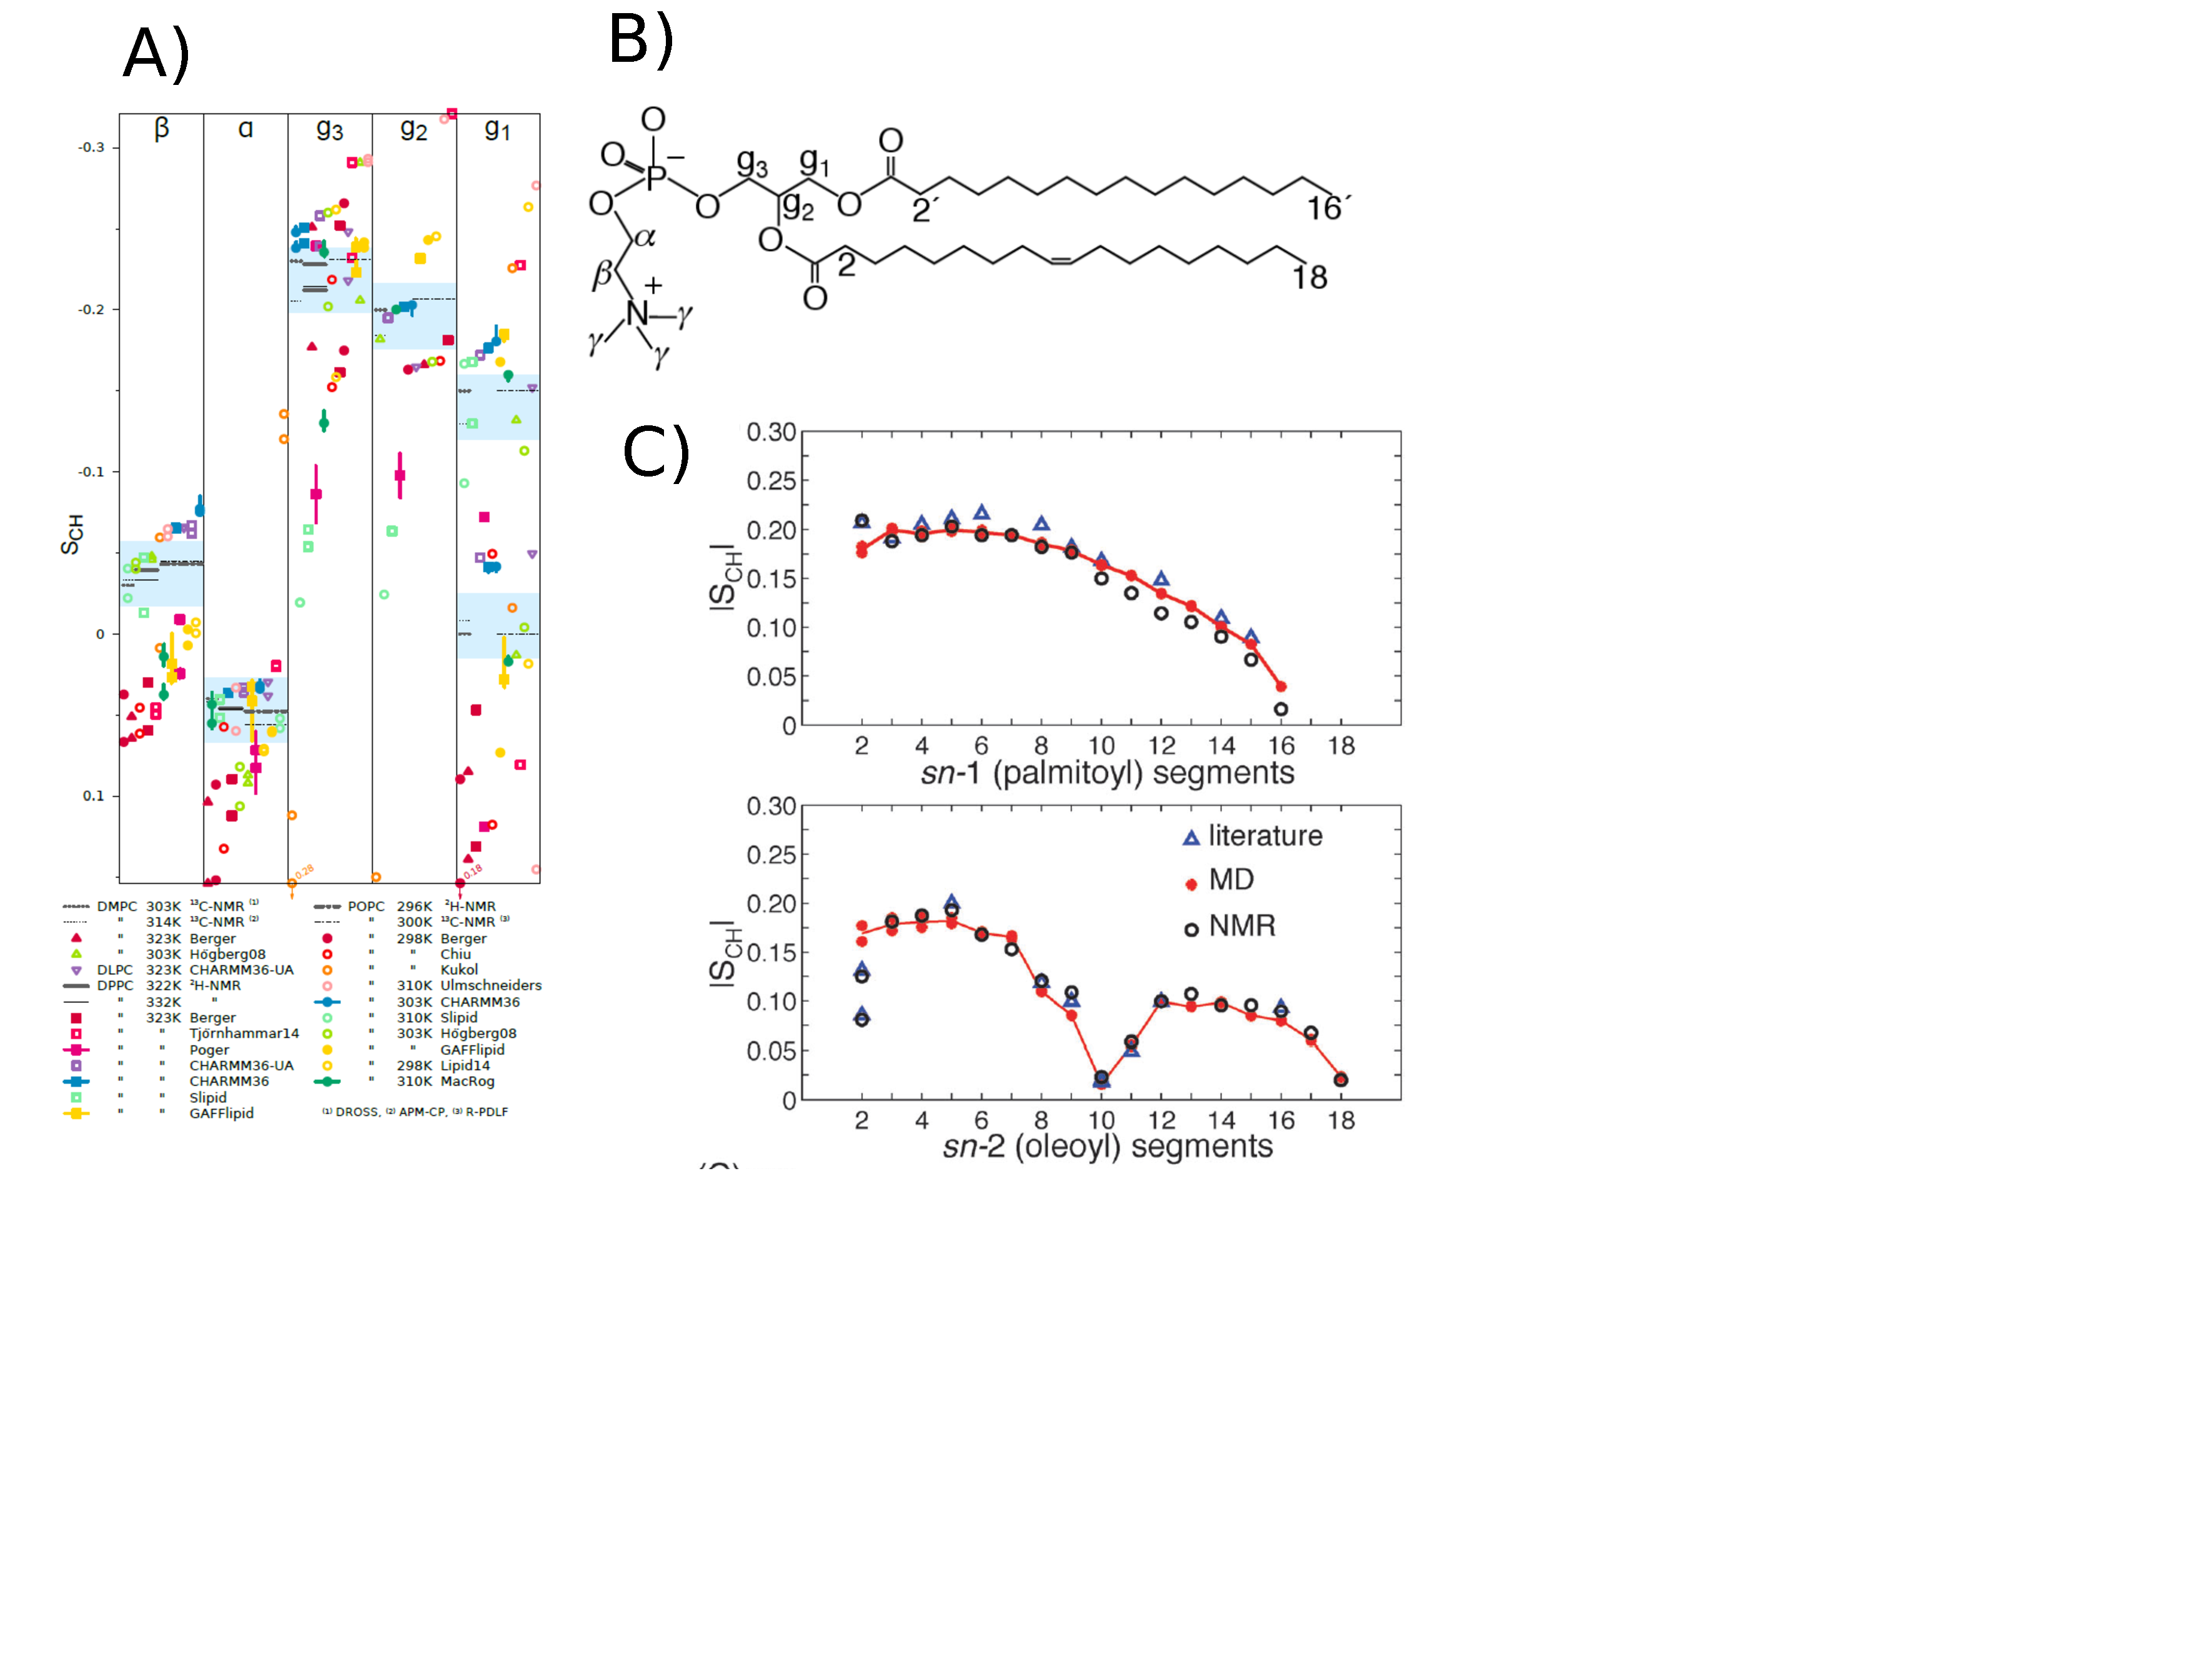
\includegraphics[width=17.2cm]{../Fig/allOPs.eps}
  \caption{\label{allOPs}
    A)  Order parameters from simulations and experimens for phosphatidylcholine headgroup and glycerol 
    backbone segments adapted from Botan et al.~\cite{botan15}. The blue shaded regions show the
    subjective sweetspots where the simulation data should fall to agree with experiments, 
    based on estimated quantitative accuracy of order parameter measurements by Botan et al.
    B) Chemical structure of 1-palmitoyl-2-oleoylphosphatidylcholine (POPC).
    C) Order parameters $|S_{{\rm CH}}|$ for POPC acyl chains 
    from $^1$H-$^{13}$C NMR at 300K (black dots)~\cite{ferreira13},
    from $^2$H NMR at 300K (blue triangles, literature)~\cite{seelig78,perly85} and 
    from MD simulations at 298K (red dots)~\cite{ferreira13}.
    The experimental values shown in A):
    DMPC 303~K \cite{gross97},
    DMPC 314~K \cite{dvinskikh05a},
    DPPC 322~K \cite{gally75},
    DPPC 323~K \cite{akutsu81},
    POPC 296~K \cite{bechinger91}, and
    POPC 300~K \cite{ferreira13}.
    The force fields in A):
    Berger \cite{berger97},
    Hogberg08 \cite{hogberg08},
    Poger \cite{poger10},
    Ulmschneiders \cite{ulmschneider09},
    Kukol \cite{kukol09},
    Chiu \cite{chiu09},
    CHARMM36 \cite{klauda10},
    GAFFlipid \cite{dickson12},
    Slipid \cite{jambeck12},
    MacRog \cite{maciejewski14},
    Tj{\"o}rnhammar14 \cite{tjornhammar14},
    Lipid14 \cite{dickson14},
    CHARMM36-UA \cite{lee14}. 
    The interactive version of this figure is available at  https://plot.ly/$\sim$HubertSantuz/72/lipid-force-field-comparison/.   
  }
\end{figure*}


Experimental order parameter data for single component lipid bilayers is very 
well available in the literature~\cite{castro07,castro08,leftin11,marsh13,ferreira13,leftin13,leftin14,botan15}. 
The amount of data, especially from $^{13}$C NMR, has been also increasing lately~\cite{castro07,castro08,ferreira13,leftin13,leftin14}.
Also changes of order parameters for all lipid segments has been measured respect to several
different conditions, like temperature \cite{??}, hydration level \cite{bechinger91,ulrich94,mallikarjunaiah11,dvinskikh05a} and
due to the presense of ions and charged objects~\cite{akutsu81,altenbach84,seelig87,scherer89}, 
cholesterol \cite{brown78,douliez95,ferreira13,leftin14} and proteins \cite{kuchinka89,roux90,leftin13}.
The comparison of order parameter responses between experiments and simulations
has not been much utilized in the literature, thus we will exemplify its potential by showing
the Na$ +$ ion effect on choline order parameters and its relation to ion partition in both, 
simulations \cite{ionpaper} and experiments \cite{akutsu81,altenbach84,seelig87,scherer89}.

In this work we discuss only order parameters directly measured from multilamellar samples 
which are closest experimental analogue to MD simulations with periodic boundary conditions. 
We do not discuss order parameters measured for other type of samples, 
e.g. bicelles~\cite{aussenac03,raffard00,sanders92}, or indirect measurements by using, e.g. relaxation
data~\cite{marbella15} since the comparison to the standard simulation setup is less straightforward.  


 

\subsection{Order parameters from $^2$H NMR experiments}\label{DopSECTION}

The absolute values of order parameters are connected to the quadrupolar splitting $\Delta \nu_Q$ 
in $^2$H NMR experiments through the equation 
\begin{equation}\label{HNMRop}
|S_{{\rm CD}}|=\frac{4}{3} \frac{h}{e^2qQ} \Delta \nu_{{\rm Q}}, 
\end{equation}
where $e$ is the elementary charge, $Q$ is the deuteron quadrupole moment and $h$ is the Planck's constant. 
The parameter $q$ is related to the largest electric field gradient and in practise its value is not known; 
therefore the static quadrupolar coupling constant $\frac{e^2qQ}{h}$ is defined, and its value measured for 
different compounds in their solid state ($\Delta \nu_Q$ measurement from the system where order parameter is known to be 1). 
In C-D order parameter measurements for lipids, it is typical to 
use the value measured for different alkenes, $\frac{e^2qQ}{h}$=170 kHz. The relation between order parameters 
and quadrupolar splittings then becomes $S_{{\rm CD}}=0.00784 \times \Delta \nu_{{\rm Q}}$.
This relation is useful as many publications report only the quadrupolar splittings. For a review and more accurate description see the work of Seelig~\cite{seelig77c}.

For $^2H$ NMR measurements the CH$_2$ segments has to be labeled with deuterium.
This can be done specifically for a certain segment or for the several segments
simultaneously~\cite{davis83,bloom91,leftin11}. In the first case, it is known that the measured
order parameter (quadrupolar splitting) is related to the labeled segment.
In the latter case several order parameters (quadrupolar splittings) are
measured which arise from all the labeled segments, however, it is not known 
which order parameter belongs to which CH$_2$ segment. Majority of the $^2H$ NMR data
in the literature is measured from samples with perdeuterated acyl chain \cite{leftin11,marsh13}
while also order parameter data from specifically deuterated lipids are available for 
several lipid types in various conditions~\cite{seelig74,seelig75,seelig77,seelig78,gally81,akutsu81,altenbach84,scherer89,kuchinka89,roux90,ulrich94,douliez95}.

\subsection{Order parameters from $^{13}$C NMR experiments}\label{CopSECTION}

The order parameter can be related to the dipolar splitting $\Delta \nu_\mathrm{CH}$ 
from $^{13}$C-$^1$H NMR experiment which is related to the effective dipolar 
coupling $d_\mathrm{CH}$ through a scaling factor depending on the used pulse 
sequence~\cite{hong95a,gross97,dvinskikh05a,ferreira13}. The effective dipolar 
coupling $d_{{\rm CH}}$ is then connected to the absolute value of order parameter through equation
\begin{equation}\label{CNMRop}
|S_{{\rm CH}}|=(\frac{D_{{\rm max}}}{2\pi})^{-1}d_\mathrm{CH},
\end{equation}
where $D_{{\rm max}} = \frac{\hbar \mu_0 \gamma_h \gamma_c}{4\pi\langle r_\mathrm{CH}^3 \rangle}$. 
$r_{{\rm CH}}$ is the C-H distance, $\mu_0$ is the vacuum permittivity, and $\gamma_h$ and $\gamma_c$ are 
the gyromagnetic constants for $^1$H and $^{13}$C nuclei. In contrast to Eq.~\ref{HNMRop}, all the parameters in 
Eq.~\ref{CNMRop} are in principle known. However, for the internuclear distance only the average $\langle r_{{\rm CH}} \rangle$ 
is known, not the third moment $\langle r^3_{{\rm CH}} \rangle$. For this reason values between 20.2-22.7 kHz are used for
$\frac{D_{{\rm max}}}{2\pi}$ depending on the original authors~\cite{hong95a,gross97,dvinskikh05a,becker05,ferreira13,ferreira15}.

In contrast to $^2$H NMR specific labeling is not needed for $^{13}$C NMR experiments due the 
natural abundance of $^{13}$C, however it could be used to enhance the signal for specific 
segment under interest~\cite{sivanandam09}. Order parameter measurements with $^{13}$C NMR are
2D experiments, the chemical shift being in the first dimension and dipolar coupling 
in the second~\cite{hong95a,gross97,dvinskikh05a,ferreira13}. The chemical shift depends on the local chemical environment and 
is different for each carbon segment. In the second dimension the dipolar coupling
(order parameter) corresponding each chemical shift value is measured, and its value 
can be connected, in principle, to each carbon segment by using the chemical shift value.  
This is straighforward for hydrocarbon segments in choline, glycerol backbone, close to the 
double bonds, and in the beginning and the end of acyl chains due to their distinct chemical 
shift values~\cite{hong95a,gross97,dvinskikh05a,ferreira13,leftin14}.
Challenges occur in the acyl chain region where chemical shift values 
of different segments are very close to each others~\cite{hong95a,gross97,dvinskikh05a,ferreira13,leftin14}. 
This issue has been solved by filtering the spectra by using partially deuterated lipids \cite{ferreira13}
and using data from simulations and previous specifically deuterated experiments to help in 
the assigment~\cite{ferreira13,leftin14}. 


\subsection{Quantitative accuracy of experimental order parameter values}\label{QUANTaccuracySECTION}

It must be stressed that $^2$H NMR and $^{13}$C NMR are fully independent experiments since the deuterium quadrupolar splitting $\Delta \nu_Q$
and the dipolar splitting $d_{{\rm CH}}$ are different physical observables. In addition, the prefactors connecting the observables to the order 
parameter (Eqs.~\ref{HNMRop} and~\ref{CNMRop}) are independently measured. Further independent experiments are performed 
by measuring the $^1$H-$^{13}$C dipolar couplings using different pulse sequences~\cite{hong95a,gross97,dvinskikh05a,ferreira13} 
when the connection between dipolar splitting $\Delta \nu_{{\rm CH}}$ and effective dipolar coupling $d_\mathrm{CH}$ is different.

The measurements of quadrupole $\Delta \nu_Q$ and dipolar $d_{{\rm CH}}$ splittings are relatively accurate, especially for quadrupolar splitting.
\todo{How accurate exactly?} 
Thus the quantitative accuracy of measured order parameters is mainly determined by the  
prefactors connecting the splittings and order parameters in Eqs.~\ref{HNMRop} and~\ref{CNMRop}. 
Since the prefactors are independently determined for the $^2$H and $^{13}$C NMR measurements,
the quantitative accuracy is best estimated by comparing the independently measured order parameter values.

These comparisons are done by several authors and generally they show a very good 
agreement~\cite{gross97,dvinskikh05a,ferreira13,botan15,leftin14}.
Botan et al. collected literature values for PC lipid choline headgroup and glycerol backbone order parameters 
and concluded that order parameters would be known with the accuracy of $\pm$0.02 for these segments in 
purified PC lipid bilayer samples~\cite{botan15} which agrees with the estimate of Gross et al~\cite{gross97}. 
Based on this Botan et al. suggested sweet spots where choline and glycerol backbone order parameters should fall in the 
simulation models, see Fig.~\ref{allOPs} A). Also acyl chain order parameters from different techniques 
are in good agreement when compared by several authors~\cite{gross97,dvinskikh05a,ferreira13,leftin14},
however the 0.02 accuracy might not be achieved for some segments.\todo{Maybe specify to which ones?}.
The comparison by Ferreira et al.~\cite{ferreira13} for POPC acyl chains is also shown in Fig.~\ref{allOPs} C). 







\subsection{Qualitative accuracy of experimental order parameter values}

When order parameter changes are measured with varying conditions, like temperature \cite{seelig74,seelig77,douliez95}, 
hydration level~\cite{bechinger91,ulrich94,mallikarjunaiah11,dvinskikh05a}, presense of ions~\cite{akutsu81,altenbach84,seelig87,scherer89}, 
cholesterol~\cite{brown78,douliez95,ferreira13,leftin14} or proteins~\cite{kuchinka89,roux90,leftin13},
the prefactors connecting the order parameters and the measured couplings in Eqs.~\ref{HNMRop} and~\ref{CNMRop} can be considered 
to be unchanged. Therefore, accuracy of the measured change is determined by the accuracy of the splitting measurement
in contrast to the prefactor in previous section. Here we refer to this as a qualitative accuracy. Due to the high resolution of
splitting measurements, especially in $^2$H NMR, the qualitative accuracy is much higher than the
quantitative accuracy discussed in previous section.

The high qualitative accuracy of order parameter measurements is demonstrated in Figs.~\ref{opIONeffect} and~\ref{opDEHYDeffect}
showing the measured changes as a function of ion concetrations and hydration level, respectively.
Systematically observed order parameter decrease of choline $\alpha$ and $\beta$ segments due to penetrating 
positive charges~\cite{akutsu81,altenbach84,seelig87,scherer89} from $^2$H NMR are shown in Fig.~\ref{opIONeffect} A).
The quadrupole splittings reported in the original work~\cite{akutsu81} and corresponding order parameters 
are shown. The clearly measurable quadrupolar splitting changes correspond order parameter changes below 0.03 and 
0.05 units for $\beta$ and $\alpha$, respectively. Systematically observed increase for choline $\beta$ and $\alpha$
segments due to decreased hydration level is shown in Fig.~\ref{opDEHYDeffect}. 
Similar increase is observed for different phosphatidycholine lipids in slightly different temperatures measured by
different groups by using both $^2$H NMR~\cite{bechinger91,ulrich94} and $^{13}$C NMR~\cite{dvinskikh05b}.
The results demonstrate the systematic changes only slightly above 0.01 units can be detected also with $^{13}$C NMR~\cite{dvinskikh05b}.

\begin{figure*}[]
%  \centering
  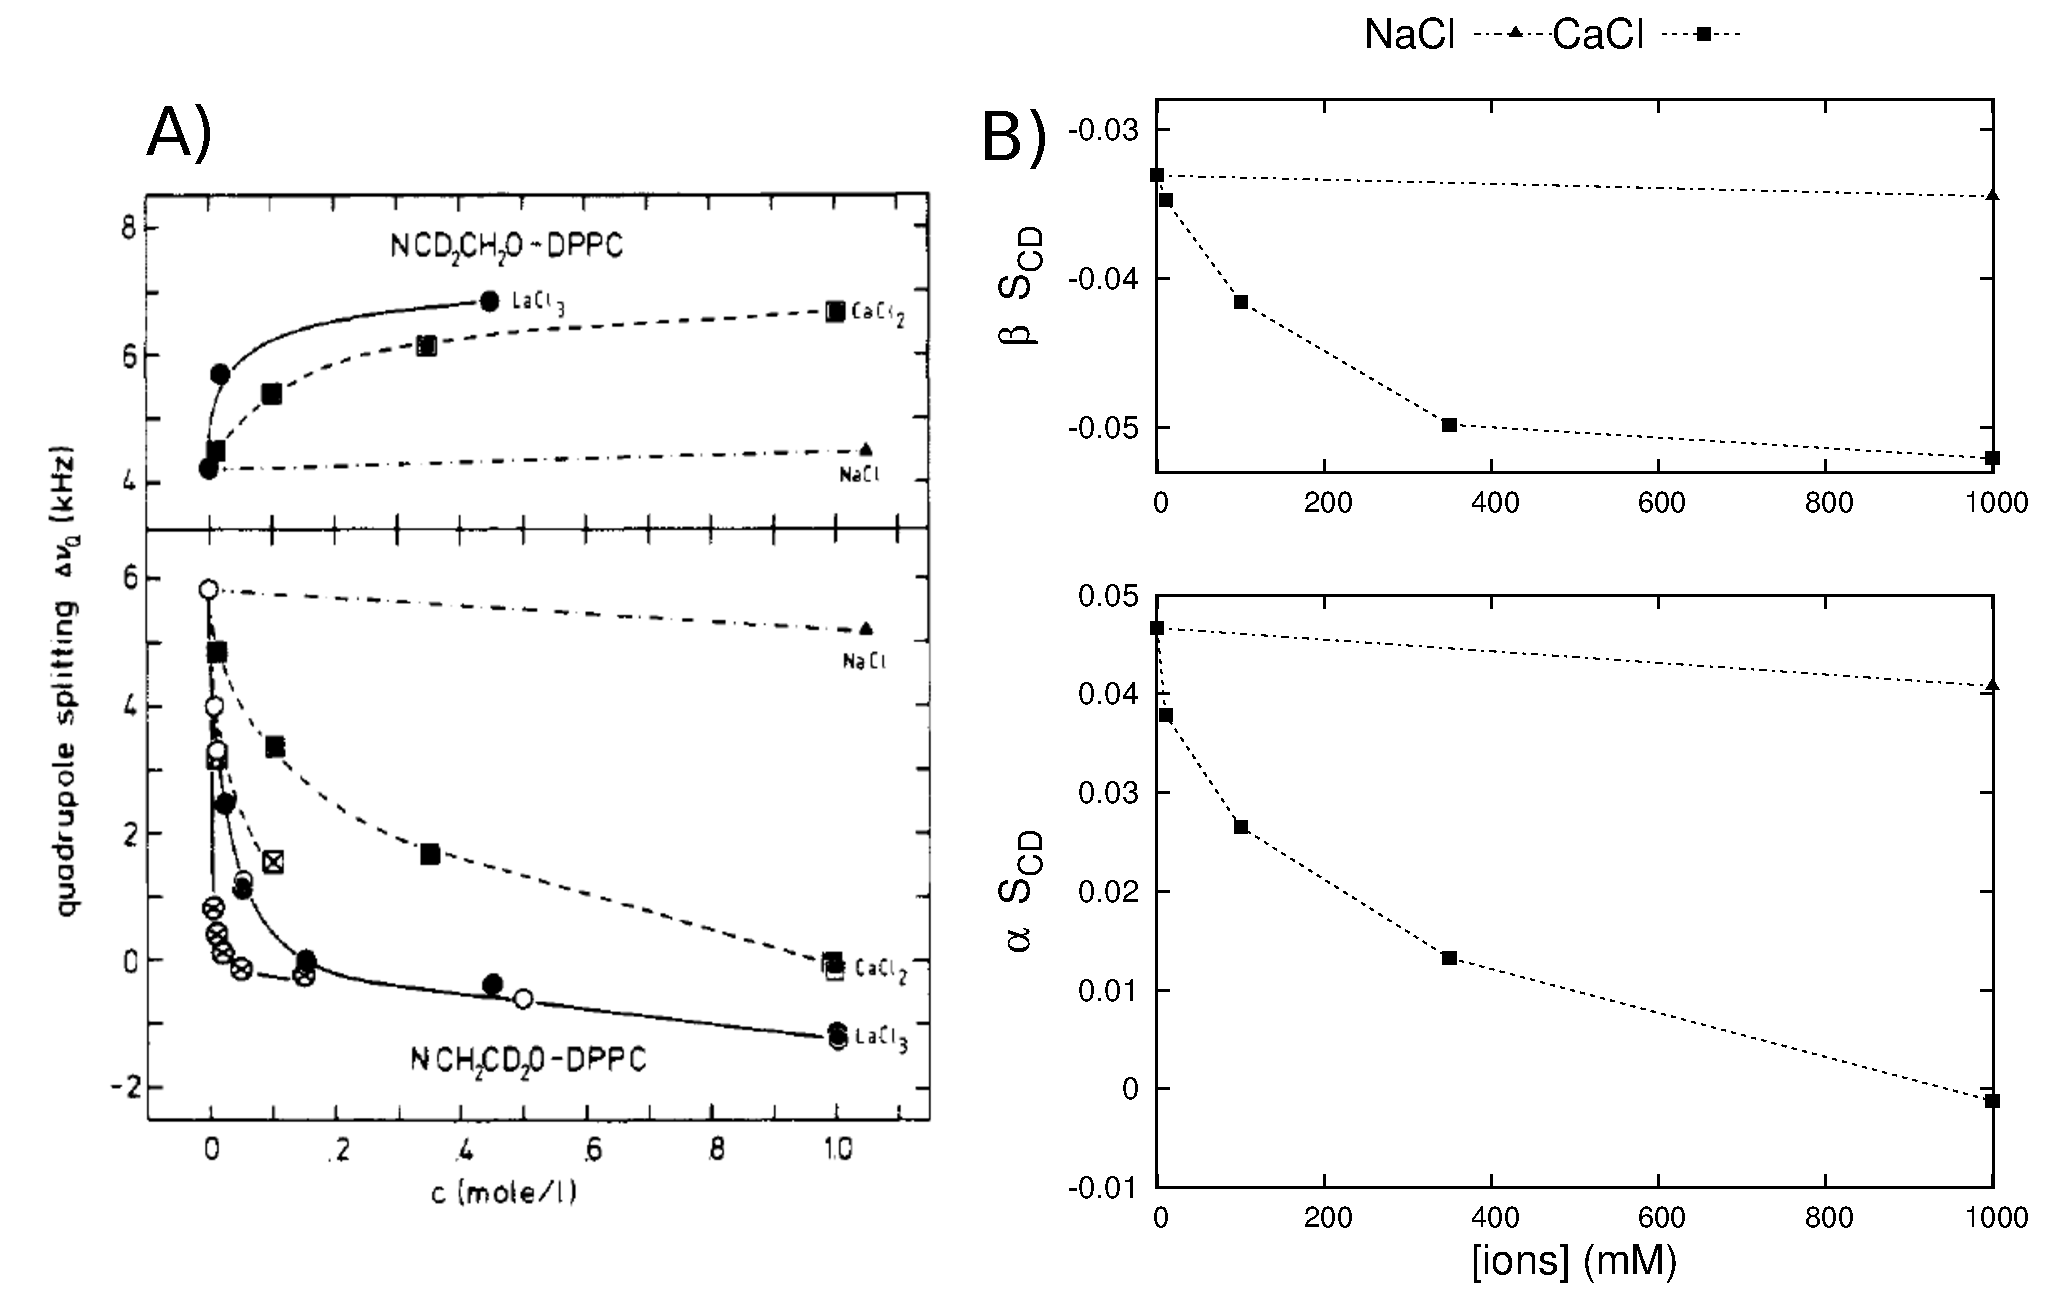
\includegraphics[width=17.2cm]{../Fig/QPandOPwithIONS.eps}
  \caption{\label{opIONeffect}
    A) Quadrupolar splittings of DPPC $\alpha$ and $\beta$ segments as a function of different 
    ion concetrations measured by Akutsu and Seelig with $^2$H NMR~\cite{akutsu81}. 
    B) The measured quadrupolar splittings with NaCl and CaCl$_2$ translated to order parameters ($S_{{\rm CD}}=0.00784 \times \Delta \nu_{{\rm Q}}$). 
    The negative sign for $\beta$ order parameter is assigned according to more recent experiments~\cite{hong95a,hong95b,gross97} 
    (see also Ref.~\cite{botan15} and Section~\ref{signSECTION}). These changes were later shown to be consistent with the 
    addition of different charges into the bilayer, and the electrometer concept was introduced to measure the amount of charge 
    incorporated in the bilayer interface~\cite{akutsu81,altenbach84,seelig87,scherer89}.
  } 
\end{figure*}

\begin{figure}[]
%  \centering
  \includegraphics[width=8.6cm]{../Fig/OrderParameterDEHYDexp.eps}
\newline
  \caption{\label{opDEHYDeffect}
    Systematic increase of phosphatidylcholine $\alpha$ and $\beta$ order parameters with decreasing hydration level,
    observed with both $^2$H NMR~\cite{bechinger91,ulrich94} and $^{13}$C NMR~\cite{dvinskikh05b}.
    The negative sign for $\beta$ order parameter is assigned according to more recent experiments~\cite{hong95a,hong95b,gross97} 
    (see also Ref.~\cite{botan15} and Section~\ref{signSECTION}).
    The choline order parameter increase is related to the P-N vector tilting more parallel to the membrane plane~\cite{botan15}
    while relation between order parameter decrease and tilting more perpendicular has been suggested~\cite{scherer89}.
  } 
\end{figure}

In conclusion, the order parameter changes can be measured with very high accuracy,
thus even very small structural changes can be observed. Molecular models are necessary
to analyze the measured changes to avoid overinterpretation from tiny changes observed in experiments.
For example, high concentration of cholesterol induces measurable changes (less than 2~kHz) to the DPPC $\alpha$ and $\beta$ 
quadrupolar splittings, however, the related structural changes are probably almost negligible~\cite{brown78,botan15}.


\subsection{Signs of order parameters}\label{signSECTION}

The $^2$H NMR~\cite{seelig77c} and standard $^1$H-$^{13}$C NMR~\cite{hong95a,gross97,dvinskikh05a,ferreira13} techniques measure 
only the absolute value of order parameter. However, two different $^1$H-$^{13}$C NMR techniques applied to eggPC~\cite{hong95a} 
and DMPC~\cite{hong95a,gross97} allow also the measurement of the sign.
The experiments report negative order parameters for almost all the segments, only $\alpha$ and $\gamma$ are positive.
Furthermore, the signs~\cite{hong95a,hong95b,gross97} and magnitudes~\cite{gally81,ferreira13,botan15} of choline headgroup 
and glycerol backbone order parameters are practically unaffected by the acyl tail contents of the bilayers. 
The results indicate that the order parameter signs for these segments can be assumed to be the same in all PC lipids in bilayer. 
On the other hand, the positive signs for g$_1$, g$_3$ and C$_2$ has been reported by Aussenac et al.~\cite{aussenac03} 
which has led to some confusion in simulation community~\cite{hogberg06,hogberg08,signPOST}. 
However, these signs are not directly measured but extracted from the model used to interpret 
$^2$H NMR order parameters from DMPC bicelles~\cite{aussenac03}. Thus, it is reasonable to conclude that 
order parameters are negative for all segments except for $\alpha$ and $\gamma$, as 
directly measured with $^1$H-$^{13}$C NMR~\cite{hong95a,hong95b,gross97}.

%Even though the sign was not measurable with $^2$H NMR, the sign was believed to be negative for acyl chains because $\theta$ was expected to fluctuate 
%around 90$^o$ leading to negative order parameters~\cite{seelig77c}. This was later confirmed by using $^{13}$C NMR measurements~\cite{hong95a}. 
%Also MD simulations always produce negative order parameters for acyl chains.

In the measurements of order parameter changes respect to varying 
conditions~\cite{seelig74,seelig77,bechinger91,ulrich94,mallikarjunaiah11,dvinskikh05a,akutsu81,altenbach84,seelig87,scherer89,brown78,douliez95,ferreira13,leftin14,kuchinka89,roux90,leftin13} 
only the absolute values are measured. However, the experiments are usually done by gradually changing the conditions and systematic 
order parameter responses are observed~\cite{akutsu81,altenbach84,bechinger91,ulrich94,dvinskikh05b,mallikarjunaiah11,ferreira13} 
(see also Figs.~\ref{opIONeffect} and~\ref{opDEHYDeffect}), indicating that sudden changes of sign are not present. 
On the other hand, large amount of bound positive charge may decrease the $\alpha$ carbon order parameter below zero
as demonstrated by the spectra measured by Altenbach and Seelig~\cite{altenbach84} for POPC with high concetrations of CaCl$_2$,
shown in Fig.~\ref{qsCACLeffect}.
\begin{figure}[]
%  \centering
  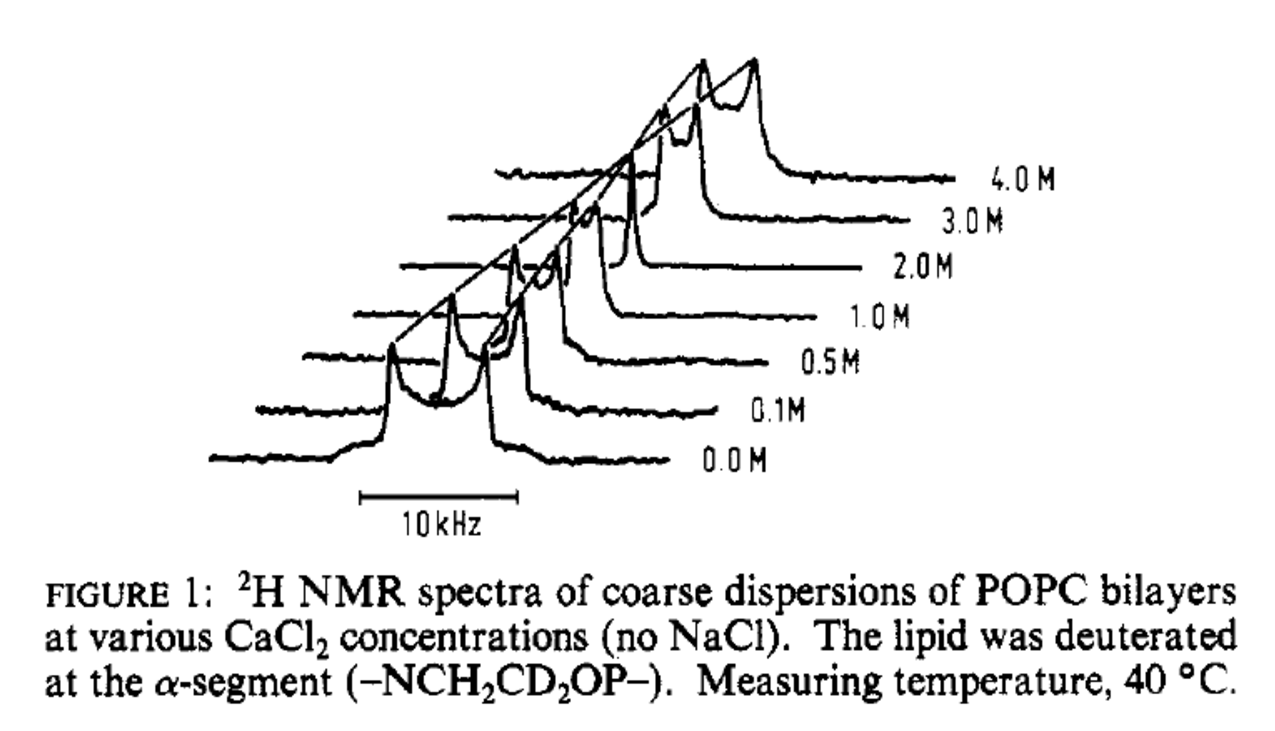
\includegraphics[width=8.6cm]{../Fig/QUADsplitCACLeffect.eps}
\newline
  \caption{\label{qsCACLeffect}
    Quadrupolar splitting $\Delta \nu_Q$ for $\alpha$ segment in POPC as a function of CaCl$_2$ concentration measured by Altenbach and Seelig~\cite{altenbach84}.
    The splitting is related to the order parameter as $S_{{\rm CD}}=0.00784 \times \Delta \nu_Q$. 
    More recent studies show that the $\alpha$ order parameter is positive in the absense of CaCl$_2$~\cite{hong95a,hong95b,gross97}.
    Thus, the most obvious interpertation is that the $\alpha$ order parameter decreases to zero when CaCl$_2$ concentration reaches 2.0M, and 
    becomes increasingly negative with further addition of CaCl$_2$. Reprinted with permission from Altenbach and Seelig, Biochemistry, 23, 3913 (1984). Copyright 1984 American Chemical Society.    
  } 
\end{figure}



\subsection{Forking of order parameters}

The order parameters for two C--H bonds in the same CH$_2$ segment are equal for the most segments in 
lipids~\cite{seelig74,seelig77,seelig78,gally81,gross97,dvinskikh05a,ferreira13}.
However, this is not the case for g$_1$, g$_3$, and  C$_2$ carbon in the \textit{sn}-2 chain segments in
a fluid PC lipid bilayer as observed with both $^2$H NMR~\cite{seelig75,seelig78,engel81,gally81} and 
$^1$H-$^{13}$C NMR techniques~\cite{gross97,dvinskikh05a,ferreira13}, see also Fig.~\ref{allOPs}.
We call this phenomena as {\it forking}, as done also previously to avoid confusion with splittings measured with NMR~\cite{botan15}.

The forking has been studied in detail with $^2$H NMR techniques by separately deuterating the 
R or S position in CH$_2$ segments to assign order parameters to correct hydrogens \cite{gally81,engel81}.
These studies also show that the forking arises from differently sampled orientations 
of the two C--H bonds, not from two separate populations of lipid conformations~\cite{engel81,gally81}.
This means that the realistic atomistic resolution molecular model has to reproduce the forking 
correctly and the isomeric positions of hydrogens must be taken into account when calculating
order parameters from simulations~\cite{botan15}.



\subsection{Order parameters from simulations}

Since all the atom coordinates are available from molecular dynamics simulations trajectory,
the order parameters can be calculated directly from the definition in Eq.~\ref{orderP}.
The ensemble average is taken over the time and all the molecules in simulation.
The hydrogen positions can be generated post-simulationally for united atom simulations without explicit hydrogens 
by creating a trajectory with added hydrogens~\cite{ollila07a,botan15}, or by using equations to directly calculate 
order parameters~\cite{tieleman97,vermeer07} based on heavy atoms positions and the known hydrocarbon geometries.
The first approach necessary for accurate structural studies since it allows the analysis of forking in contrast to the latter.

The difference in the analysis methods for the forked segments is most likely reason for different choline and glycerol
backbone order parameters reported for the same models by different authors~\cite{poger12,botan15}.
Also different order parameters for C--H segments attached to double bond are reported for the same model~\cite{bachar04,ollila07a}
due to bug in widely used version of {\it g\_order} program in the Gromacs package.
The {\it g\_order} program also prints -S$_{{\rm CH}}$ which is most likely the reason to
the reported positive order parameters for acyl chains in some studies~\cite{ekkabut07}.
When these technical issues are taken into account, the different order parameters calculations from simulations are 
in good agreement.

The statistical error for order parameters is estimated by using the error of the mean for time blocks~\cite{ollila07a},  
independent simulations~\cite{poger12} and different lipids~\cite{botan15}. All these approaches gives the maximum error 
bars of $\sim \pm$0.01.

It was recently pointed out that the sampling of individual dihedral angles might be very
slow compared to the typical (100~ns) simulation timescales~\cite{vogel12}.
This result raises a question if the molecules sample the full phase phase
during typical simulation time scales. On the other, another recent study showed
that the slowest rotational auto-correlation function observed (for g$_1$ segment) 
in the Berger model reached a plateau ($S_\mathrm{CH}^2$) after $\sim$200~ns
and its relaxation was significantly too slow compared to NMR relaxation experiments~\cite{ferreira15}. 
This indicates that the typical simulation times are long enough for full conformational 
phase space sampling for the models with realistic dynamics~\cite{ferreira15}.



\subsection{Comparison between order parameters from simulations and experiments}

The acyl chain order parameters are compared between simulations and experiments since the early days of lipid bilayer 
simulations~\cite{ploeg82,egberts88,stouch93,egberts94,essex94,robinson94,hyvonen95,kothekar96,tieleman96,shinoda97,berger97,tieleman97,klauda08b}. 
Good agreement has been generally found~\cite{berger97,hogberg08,poger10,ulmschneider09,kukol09,chiu09,klauda10,dickson12,jambeck12,chowdhary13,maciejewski14,tjornhammar14,dickson14,lee14}.
except for C$_2$ segment in {\it sn-2} chain which has low magnitude and significant forking in all PC lipids, in constrast to C$_2$ in 
{\it sn}-1~\cite{seelig74,seelig75,gross97,dvinskikh05a,ferreira13}, for example see Fig.~\ref{allOPs} C). 
This feature is, however, not analyzed or not reproduced for several lipid models~\cite{hogberg08,siu08,chiu09,kukol09,ulmschneider09,jambeck12,dickson12,chowdhary13,tjornhammar14,maciejewski14}
while some models report the lower magnitude but the forking is not reproduced correctly or analyzed~\cite{siu08,klauda10,chowdhary13,dickson14}.
The united atom CHARMM36 is really close the experimental results~\cite{lee14}.

Also acyl chain order changes with varying conditions are compared between simulations and experiments
by several authors. Experimentally observed order parameter increase with cholesterol 
concentration~\cite{dufourc84,lafleur90,douliez95,urbina95,vermeer07,ferreira13} and dehydration~\cite{mallikarjunaiah11,dvinskikh05b} 
is observed also in simulations~\cite{mashl01,hogberg06,vermeer07,zhu07,lim12,ferreira13,jambeck13,madej15},
as well as the temperature induced order parameter decrease~\cite{douliez95,zhuang14}.
More careful comparison reveals, however, that the temperature and dehydration effects are slightly underestimated in simulations 
compared to experiments~\cite{hogberg06,zhuang14}. Also cholesterol effect to DMPC bilayer is underestimated in CHARMM36 model~\cite{lim12},
while Slipids~\cite{jambeck13} and Amber Lipid14~\cite{madej15} models show satisfactory agreement.
The comparison of Berger/H{\"o}ltje~\cite{berger97,holtje01} based model to the extensive data set with various POPC/cholesterol mixtures shows a 
good agreement with experiments for low cholesterol concetrations, however, with 34\% and higher cholesterol concentrations the agreement gets worse~\cite{ferreira13}. 
Recent comparison of the Amber Lipid14 model to the same data shows signifincantly better agreement~\cite{madej15} as also
shown in Fig.~\ref{cholTAILmadej}. The orientation of cholesterol ring structure is reasonable in all models \cite{vermeer07,lim12,ferreira13,madej15}, 
however, the cholesterol acyl chain has too low order parameters in Berger/H{\"o}ltje~\cite{berger97,holtje01} based model and 
too much forking in Amber Lipid14~\cite{madej15} while CHARMM36 reproduces experiments well~\cite{lim12}. 
\begin{figure*}[]
%  \centering
  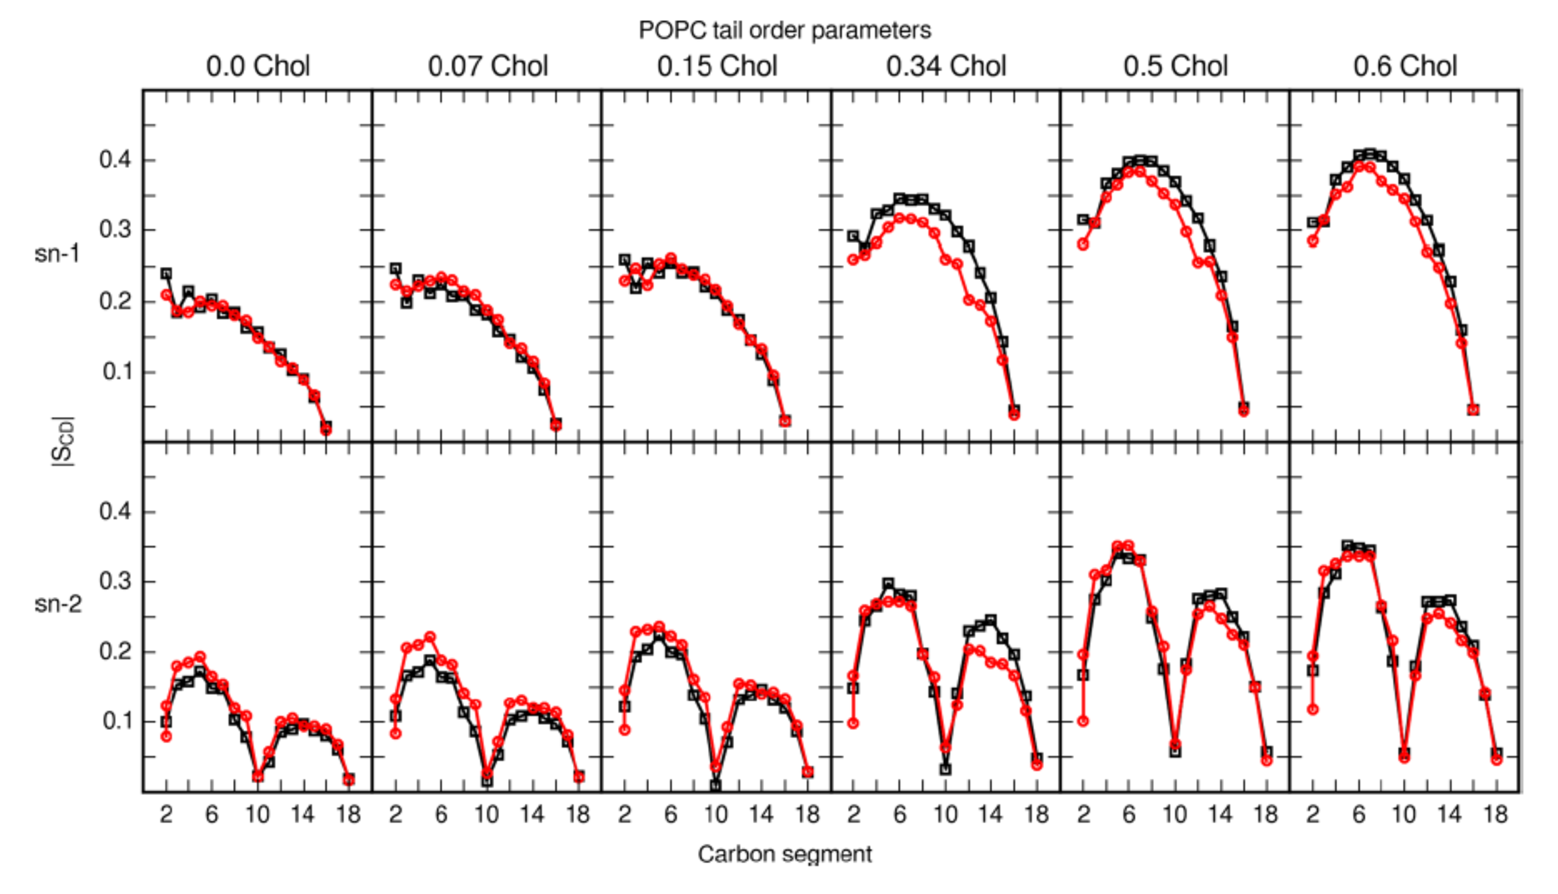
\includegraphics[width=8.6cm]{../Fig/cholTAILmadej.eps}
\newline
  \caption{\label{cholTAILmadej}
    Cholesterol effect on acyl chain order parameters compared between ? model \cite{madej15} and experiments \cite{ferreira13}.
    The agreement with experiments with this model is significanly better than Beger/H{\"o}ltje based model compared by 
    Ferreira et al. \cite{ferreira13}.
  } 
\end{figure*}


The acyl chain order parameter decrease due to double bonds is generally reproduced by different simulation 
models~\cite{hyvonen97,hyvonen97b,feller97,saiz01,huber02,feller02,bachar04,rog04,hyvonen05,ollila07a,dickson12,klauda10,klauda12,ferreira13,jambeck13,lee14,dickson14}. 
Especially good agreement often achieved for oleyl chain in POPC bilayer with one {\it cis} double bond is demonstrated in Fig.~\ref{allOPs} C).
Also the further order parameter decrease due to multiple double bonds (polyunsaturation)~\cite{hyvonen97,hyvonen97b,saiz01,huber02,feller02,bachar04,hyvonen05,ollila07a,klauda12} 
is usually well reproduced, as demonstrated in Fig. \ref{polyunsat} for Berger~\cite{berger97} based model with double bond description by Bachar et al.~\cite{bachar04}.
Also difference between {\it cis} and {\it trans} double bonds can be reproduced in MD simulations \cite{kulig15b}.
\begin{figure}[]
%  \centering
  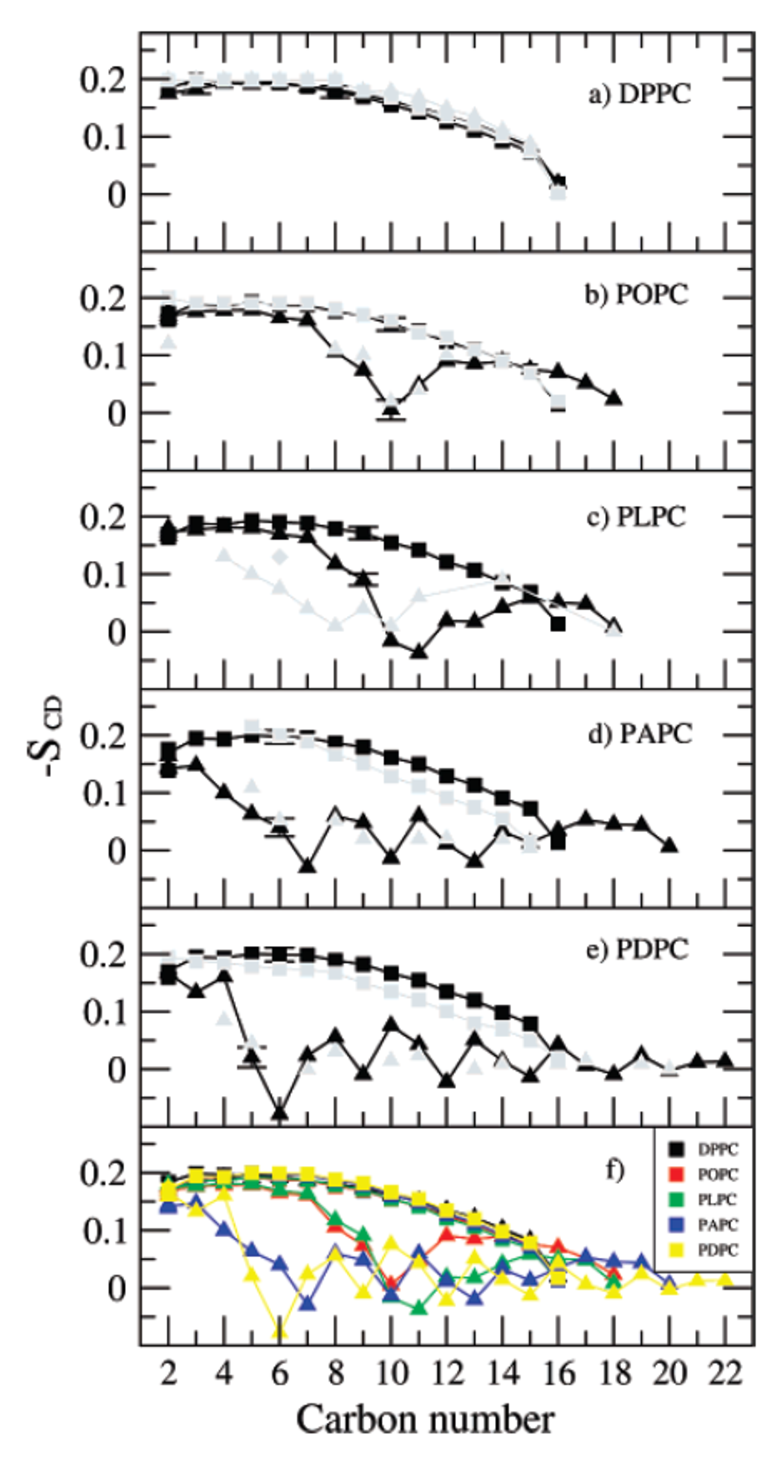
\includegraphics[width=8.6cm]{../Fig/polyunsat.eps}
\newline
  \caption{\label{polyunsat}
   Figure comparing order parameters in polyunsaturated acyl chains between simulations and 
   experiments adapted from~\cite{ollila07a}.
   Order parameters for the sn-1 (squares) and sn-2 (triangles)
   chains of (A) DPPC, (B) POPC, (C) PLPC, (D) PAPC, and (E) PDPC.
   Simulation results are shown in full black, and experimental results
   for comparison in gray. Additionally, part F summarizes the data for
   all bilayers from the simulations. Experimental order parameters were
   chosen for comparison as follows. The order parameters for DPPC (T=323K) 
   are based on studies by Petrache et al. \cite{petrache00} whereas the
   experimental S$_{{\rm CD}}$ values for PDPC and for the sn-1 chain of POPC (T=310 K) 
   are based on studies by Huber et al. \cite{huber02} For the sn-1 chain of
   PDPC, the data set at 310 K is obtained by linearly interpolating
   between data at 303 and 323 K, whereas for the sn-2 chain the data at
   303 K are presented \cite{huber02}. Experimental values for the sn-2 chain of POPC
   are based on studies by Seelig et al. \cite{seelig78} A single experimental value is
   available also for the sn-2 chain of the PLPC bilayer at 313 K
   (diamond) \cite{baenziger91} to compare with our simulated order parameters for PLPC.
   Together with PLPC, there are also experimental results for PiLPC (T=313K) \cite{baenziger91}. 
   Experimental order parameters for the sn-1 and sn-2 chains
   of PAPC (T=303 K) are based on quadrupole splittings measured by
   Rajamoorthi et al. \cite{rajamoorthi91}. For the sn-1 chain the monotonic decrease through
   the acyl chain is expected. For the sn-2 chain, values are fitted such
   that the agreement is as good as possible.
  } 
\end{figure}


In contrast to acyl chains, the glycerol backbone and choline order parameters are not routinely
compared between simulations and experiments. In most comparisons the experimentally available sings,
stereospecific labeling and high accuracy are not fully exploited~\cite{shinoda97,hogberg06,klauda10,poger12,dickson12,botan15,hogberg08,kapla12}.
These issues were recently dicussed by Botan et al. who also compared order parameters 
between 13 different simulation models and experiments~\cite{botan15}. The results, shown also in Fig.~\ref{allOPs} A),
reveal significant differences between models and experiments, and none of the available models
reproduces all order parameters within experimental error.
On the other hand, experimentally observed choline order parameter increase and decrease with 
dehydration~\cite{bechinger91,ulrich94,dvinskikh05b} and cation penetration~\cite{akutsu81,altenbach84}, 
respectively, were reproduced in simulations~\cite{botan15,ionpaper}.
However, especially the effect induced by Na$^+$ ion penetration is strongly overestimated
in most models which arises most likely from artificially high partition coefficient~\cite{ionpaper},
as also demonstrated in Fig.~\ref{changesDUEna}.
The effect of cholesterol on glycerol backbone and choline was overestimated
by the Berger/H{\"o}ltje based model while CHARMM36 and MacRog performed better~\cite{botan15}. 
\begin{figure}[]
%  \centering
  \includegraphics[width=8.6cm]{../Fig/changesDUEna.eps}
\newline
  \caption{\label{changesDUEna}
    Changes in choline order parameters (left column) and ion density distributions (right column)
    as a function of NaCl concentration. Significant order parameter
    reduction and Na$^+$ partition is observed with Berger model while only modest order parameter change
    and ion parition observed with CHARMM36. The results are in line with the electrometer concept
    connecting the ion partition and choline order parameters changes~\cite{akutsu81,altenbach84,seelig87,scherer89}.
    Consequently, the results show that Na$^+$ partition is significantly overestimated in the Berger model. 
    For more discussion see \cite{ionpaper}.
  } 
\end{figure}

In conclusion, the acyl chain order parameters and their qualitative changes are 
generally well described in atomistic MD models, except for C$_2$ segment in {\it sn}-2.
However, all models have difficulties with varying severity to describe the glycerol backbone
and choline order parameters.



\subsection{Interplay between simulations and NMR order parameters: Validation and interpretation}

This important structural fingerprint is
related to the different conformations between carboxyl segments in the beginning of chains~\cite{schindler75}.

As reviewed here, the order parameters can be measured with high accuracy for each hydrocarbon segment in lipid
in bilayer and the values are available in the literature for wide range of different lipids in different conditions.
Thus, the experimental order parameters give very detailed and local information about the orientations
sampled by each C--H bonds in the lipid bilayer system. The order parameters can 
be also calculated from MD simulations with high accuracy and compared to the experiments.
If the order parameters agree within experimental error, the simulated structures can considered as
an structural intepretation for order parameter experiments. On the other hand, if the agreement is not good, 
the simulation is sampling incorrect structures.

As discussed in the previous section, the order parameters for acyl chain region from MD simulations generally 
agree well with experiments (except for the C$_2$ segment in the {\it sn}-2 chain). Thus, the acyl chain structure 
is most likely realistic in simulations and they can used for structural interpretation for this region. 
This is a significant advancement to the traditional structural models build based on the 
fittings to the order paramters~\cite{seelig74,schindler75,seelig78,baenziger91}. The dynamical visualization of simulation trajectory immediately 
reveals very dynamical nature of acyl chains, rapidly sampling large amount of different conformations 
(for dynamics see the Section~\ref{dynamicsSECTION}). These videos published by several authors in supplementary information~\cite{??}
gives significantly better intuitive understanding of dynamical nature of lipid bilayers compared to the static ones from 
traditional models. Since the lipid bilayers can be considered as a simplistic models for cell
membranes and other biological lipid layers, this understanding has significant impact on
biophysics and biochemistry. 

Also the order parameter changes with changing conditions are qualitatively reproduced in the acyl chain region, 
however the systematic quantitative comparison of changes is rare~\cite{ollila07a,ferreira13,madej15}.
The MD simulations have been especially useful to explain the origin of order parameter decrease
due to {\it cis} double bonds in the acyl chain~\cite{feller02,huber02,eldho03,stillwell03,gawrisch03,bachar04,ollila07a}. The order parameter decrease might arise
from reduced order of the chain or from the changed average $\theta$ angle in Eq.~\ref{orderP}.
From NMR experiments alone it was impossible to judge which is the correct explanation for
the decreased order parameters due double bonds~\cite{feller02,huber02,eldho03,stillwell03,gawrisch03}. Several simulation studies by different
authors using different models has showed that the decreased order parameter order parameter due to {\it cis} double
bonds can be reproduced by introducing proper dihedral potentials next to double bonds,
and due to the fexility of these dihedrals the polyunsaturated acyl chain becomes more flexible and
the order is reduced~\cite{feller02,eldho03,stillwell03,gawrisch03,bachar04,ollila07a}. 
These studies concluded that order parameter decrease due to double 
bonds arises from genuine disorder of the chain, not from the changes in average angle~\cite{stillwell03,gawrisch03}.
This is a prime example of the case where MD simulations have significant advance over more traditional 
modeling approaches~\cite{stillwell03}.

The increase of acyl chain order parameters and related bilayer thickening due to addition of cholesterol 
is also qualitatively reproduced by simulations giving also intuitive visualizations for these effects~\cite{ferreira13,madej15}. 
However, quantitative comparison reviewed in previous section revels that some models do not reproduce the 
acyl chain order parameters within experimental error in cholesterol mixtures \cite{lim12,ferreira13}.
This indicates that these models are not yet accurate enough to give atomistic resolution interpretation
to delicate lipid cholesterol interactions which are known to induce liquid-ordereded and liquid-disordered
phase coexistence \cite{ipsen87}. The recent Amber model \cite{madej15} seems promising in this respect, see also Fig. \ref{cholTAILmadej}. 

%Thus it is not clear if currect simulations
%can be used to, e.g. intepretate atomistic resolution acyl chain ordering due to dehydration which has been
%suggested to play an important role in hydration repulsion \cite{??}.

Simulation studies have also predicted changes in the acyl chain region which are yet to be experimentally 
confirmed, e.g. order parameter decrease due to lipid oxidation and changes in order parameter sign in oxidized 
acyl chain~\cite{ekkabut07}. %A new experimental data can confirm if these predictions can be verified. 


As discussed in the previous section, simulations models are not able to reproduce the glycerol backbone 
and choline headgroup order parameters within experimental error~\cite{botan15} in contrast to acyl chains.
Thus, even the state of the art simulation models are not able to resolve the sampled atomistic resolution
structure of these segments which has been also tremendeous challenge to the more traditional models~\cite{gally75,seelig77,strenk85,akutsu91,bruzik97,Semchyschyn04}.
Consequently, the conclusions made from MD simulations which depend on atomistic resolution structure
of energetics of these segments should be taken with extreme caution.
On the other hand, the qualitative response of choline $\alpha$ and $\beta$ order parameters to the dehydration 
and penetrating ions (increase and decrease, respectively) was correctly reproduced by several models, 
despite of the incorrect structure in fully hydrated lipid bilayer~\cite{botan15,ionpaper}.
These changes could be related with the changes of P--N vector angle respect to the membrane normal as 
suggested previously in~\cite{scherer89}: the tilting of P--N vector more parallel to membrane plane with
dehydration leads to the increase of choline order parameters~\cite{botan15} and {\it vice versa} with penetrating ions~\cite{ionpaper}.
\todo{The analysis with ions not actually done yet!}
The widely used Berger/Höltje model significantly overestimates the structural effects due to cholesterol 
in the glycerol backbone and choline regions~\cite{ferreira13,botan15} which seems to be the 
case also for Lipid14~\cite{madej15}.

The recent progress in the NMRlipids collaboration has shown that simulations confirm the electrometer 
concept suggested by Seelig et al. in a serie of classical publications~\cite{akutsu81,altenbach84,seelig87,scherer89}: 
the decrease of $\alpha$ and $\beta$ order parameters is a measure of 
charge penetrated in PC lipid bilayer~\cite{ionpaper}, see also Fig,~\ref{changesDUEna}. The concept gives a 
direct and quantitative route to compare charge binding into PC lipid bilayers between simulations
and experiments through the choline order parameters~\cite{ionpaper}. While experimental results show 
only very weak or negligible Na$^{+}$ binding, some simulation models predict significantly stronger
binding, see~\cite{ionpaper} and Fig.~\ref{changesDUEna}. This is a serious artefact since specific cation binding 
makes a lipid bilayer positively charged, which has a potential to lead incorrect conclusion when interactions with
charged objects are studied. Thus the numerous conclusions from simulation studies with strongly binding 
Na$^{+}$ has to be taken with extreme caution. In contrast to monovalent ions the Ca$^{2+}$ and other multivalent ions
significantly partition to PC bilayers~\cite{cevc90,akutsu81,altenbach84}. This is also seen in simulations, however, the structural
effects are overestimated at least in the Berger model~\cite{ionpaper}. The CHARMM36 behaves more realistically, 
however, more careful simulation studies are needed to conclude if some of the existing models in capable to correctly
reproduce PC ion interactions \cite{ionpaper}. 

In conclusion, the atomistic resolution MD simulations are invaluable in understanding the 
structural details and their changes in acyl chain region, especially for double bonds.
However, serious artefacts are possible, or even likely, in simulations studies where choline or
glycerol backbone structure, or cation binding are important.


\section{C-H bond rotational dynamics from spin relaxation rates and simulations}\label{dynamicsSECTION}

%\noindent {\bf Here will be described:}\\[0.1cm]

%\noindent How the rotational dynamics measured by using NMR relaxation experiments. \\
%How the relaxation experiments are connected and compared with simulations. \\
%What can be learned and what has been learned about the rotational dynamics from the comparison between spin relaxation and simulations \\[0.5 cm]

\todo{This is the first sketch of this section. A lot of references should be added, the text should polished,
things should be added and checked and figures should be improved. However, the main strucutre and idea of the section should be visible.}

\subsection{Definition and properties of rotational autcorrelation function}
The second order auto-correlation function for the reorientation of the C--H chemical bond axis is defined as \cite{Lipari82}
\begin{equation}\label{gt}
g(\tau) = \langle P_2[\vec{\mu}(t)\cdot\vec{\mu}(t+\tau)]\rangle,
\end{equation} 
where $P_2$ denotes the second Legendre polynomial, $P_2(\xi) = 1/2 (3\xi^2 - 1)$, $\vec{\mu}(t)$ is the unitary vector having the 
direction of the C--H bond at time $t$, and the angular brackets denote a time-average. This autocorrelation is usually chosen
to describe the C--H bond rotational dynamics since it is connected to the experimentally measurable spin relaxation rates 
through its Fourier transformation called spectral density
\begin{equation}\label{FT}
j(\omega) =  2\int_0^{\infty} \cos(\omega \tau) g(\tau) d\tau.
\end{equation}
In this review we focus only on experiments measured from multilamellar samples with randomly oriented sheets, 
thus only the second order auto-correlation function is needed~\cite{??}. 

In randomly oriented multilamellar samples the auto--correlation function of bond orientations always decays to zero with
long enough time scales. However, the relaxation timescales can be divided to two distinct timescales.
First the relaxation processes shorter than microsecond timescales occurs when lipid molecules are reorienting
in the lipid bilyer but are not essentially moving between lipid bilayer regions with different orientations.
Then with larger than microsecond timescales the movement between differently oriented bilayer regions
decays the rotational correlation function to zero. In addition, MAS experiments the sample spinning
causes lead orientaitional relaxation in kHz region. The full auto--correlation decaying to zero 
is illustrated in Fig.~\ref{correlationF}. Due to the timescale separation the correlation function can 
be written as~\cite{Nowacka10}
\begin{equation}\label{corrF}
g(\tau)=g_{\rm{f}}(\tau) g_{\rm{s}}(\tau);
\end{equation}
$g_{\rm{f}}(\tau)$ describes the decay of $g(\tau)$ due to fast molecular motions and $g_{\rm{s}}(\tau)$ contains the contribution from slower motions
\begin{equation}\label{MAS}
g_{\rm{s}}(\tau)= e^{- \frac{\tau}{\tau_{\rm{s}}}} \bigg[ \frac{2}{3}\cos(\omega_R \tau) + \frac{1}{3}\cos(2\omega_R \tau)\bigg],
\end{equation}
where $\tau_s$ is a correlation time due to slower isotropic molecular motions originating from the diffusion between bilayers 
with different orientations of their principal symmetry axis, and the cosine terms are the contribution from magic angle spinning 
of the sample, rotating at $\omega_{\rm{R}}/2\pi$ cycles per second~\cite{Hirschinger06}, typically in the kHz frequency range. 

%We expect 
%a two step model behavior \cite{Hal81:1928} of the correlation function $g(\tau)$ as illustrated in Figure \ref{correlation_function} 
%and described as follows. First, $g(\tau)$ will decay due to fast anisotropic molecular motions to a plateau value equal to the square 
%of the order parameter $S_{\rm{CH}}=\langle P_2(\cos\theta)\rangle$, where $\theta$ denotes the angle between the C--H bond and the bilayer 
%normal. $|S_{\rm{CH}}|$ can be accurately measured by a number of NMR techniques~\cite{Lef11:818}. 
%At much longer time scales,  $g(\tau)$ will then oscillate due to MAS and relax to zero because of slower isotropic motions. Since Pake 
%pattern line shapes with splittings $\Delta\nu$ from a few to tens of kHz can be measured for lipid bilayers \cite{Lef11:818,Dav83:117}, 
%the time scale for these isotropic slow motions must be much slower than $1/\Delta\nu$, or deviations from such Pake patterns would be 
%detectable~\cite{Jag87:167}. Thus $g(\tau)$ will only start to decay from the plateau $S_{\rm{CH}}^2$  at time scales well above $\mu$s.


The order parameter measurements with $^2$H NMR and $^{13}$C NMR measure the bond order after the relaxation
of rotational motion inside the bilayer plane but before the relaxation between different bilayer orientations,
as illustrated in Fig.~\ref{correlationF}. In typical molecular dynamics simulations with periodic boundary conditions
the lipid molecules are restricted to single bilayer orientation and also the timescales are currently
typically below microsecond. In these simulations the auto--correlation function in Eq.~\ref{gt} decays
to the square of order parameter in Eg.~\ref{orderP} in bilayers with planar symmetry, i.e. no microscopic phase separation of defects present.
Also this is illustrated in Fig.~\ref{correlationF}.
\begin{figure}[]
%  \centering
  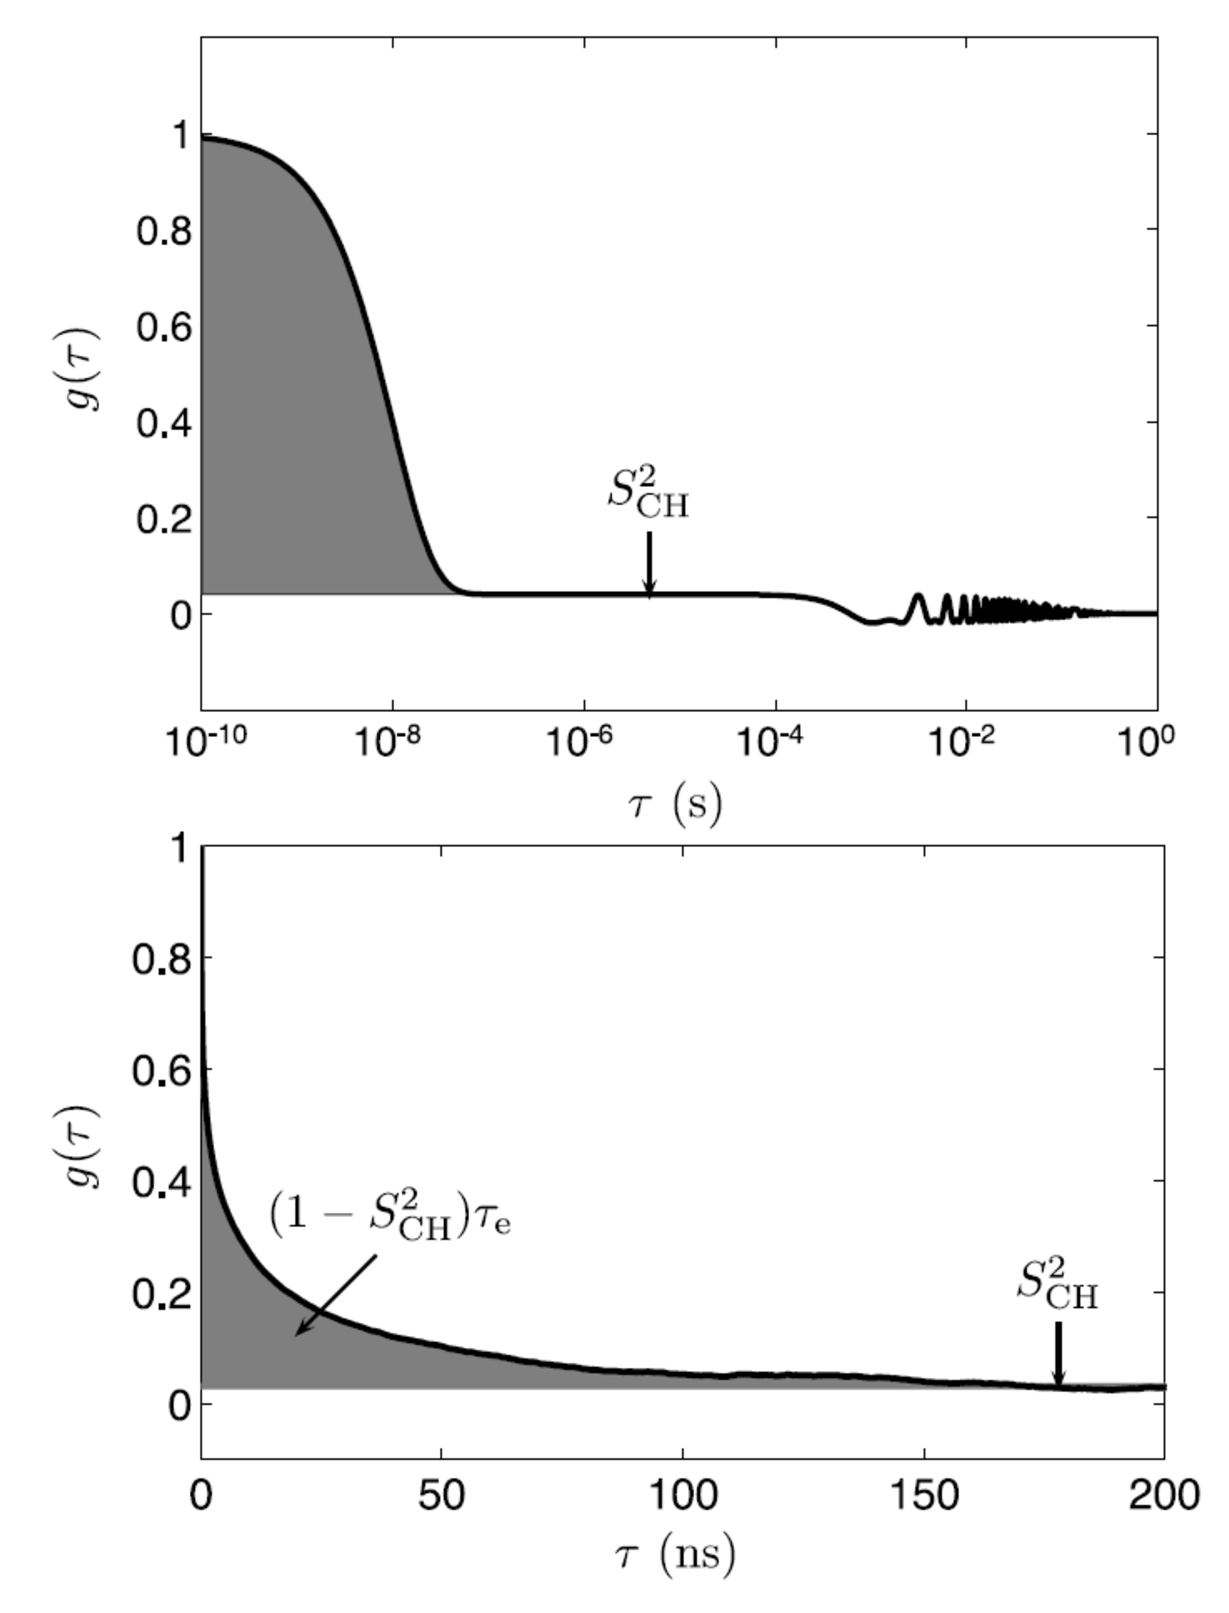
\includegraphics[width=8.6cm]{../Fig/correlationF.eps}
\newline
  \caption{\label{correlationF}
    (Top) Illustration of the auto-correlation function $g(\tau)$ and effective
    correlation time $\tau_e$ for a $ 13$C–H bond in a lipid bilayer in MAS experiment (x--axis with logarithmic scale).
    Plateau after short timescale relaxation processes ($g(\tau)_f$) is shown between roughly 10$^{-7}$s and 10$^{-4}$s.
    After this timescale the slow relaxation processes ($g(\tau)_f$) and oscillation due to MAS (Eq. \ref{MAS}) are shown.
    (Bottom) Example of $g(\tau)$ from a united-atom MD simulation of a POPC bilayer in excess water, 
    illustrating the decay towards $S^2_{{\rm CH}}$ (x--axis with linear scale). This represents the $g(\tau)_f$ in Eq. \ref{corrF} and 
    decrease to the plateau in the top figure.
    The effective correlation time $\tau_e$ is equal to the area in gray scaled by $(1−S^2_{{\rm CH}})^{−1}$.
    Figure adapted from \cite{ferreira15}
  } 
\end{figure}

The rotational correlation function describes how long does it take for a single molecule
on average to sample the conformations. The effective correlation time 
\begin{equation}\label{effCTdef}
\tau_{e}:=\int_0^{\infty} \frac{g_{\rm{f}}(\tau)-S_{\rm{CH}}^2}{1-S_{\rm{CH}}^2} \mathrm{d}\tau
\end{equation} 
can be used as an intuitively useful single parameter to describe this time. 
The larger this parameter is, the longer it takes in average to sample the conformations related to the
bond. With this definition the area between the correlation function and its pleateau becomes $(1-S_{\rm{CH}}^2)\tau_{e}$.

\subsection{Detecting C--H bond dynamics experimentally}

The most used parameter to detect the C--H bond dynamics experimentally in time scales comparable to simulations
are the spin-lattice relaxation rates $R_1$ from deuterium labels and $^{13}$C. 
$R_1^{C}$ measured from $^{13}$C is connected to the spectral density (Eq.~\ref{FT}) through the equation
\begin{equation}\label{R1C}
R_{1}^{C}=\frac{D_{\rm{max}}^2N_{\rm{H}}}{20}\bigg[j(\omega_{\rm{H}}-\omega_{\rm{C}})+3j(\omega_{\rm{C}})+6j(\omega_{\rm{C}}+\omega_{\rm{H}})\bigg],
\end{equation}
where $\omega_{\rm{C}}$ and $\omega_{\rm{H}}$ are the Larmor angular frequencies of $^{13}$C and $^1$H respectively, 
$N_{\rm{H}}$ is the number of bound protons and $\frac{D_{\rm{max}}}{2\pi}\approx$22 kHz as in section~\ref{CopSECTION}.
%is given by
%\begin{equation}
%d_{\rm{CH}}=-\frac{\mu_0\hbar\gamma_{\rm{H}}\gamma_{\rm{C}}}{4\pi\langle r_{\rm{CH}}^3\rangle},\nonumber
%\end{equation}
%where $\mu_0$ is the magnetic constant or vacuum permeability, $\hbar$ is the reduced Planck constant, 
%$\gamma_{\rm{C}}$ and $\gamma_{\rm{H}}$ are the gyromagnetic constants of $^{13}$C and $^1$H, respectively, 
%and $\langle r_{\rm{CH}}^3\rangle$ is the average cubic length of the C--H chemical bond. $d_{\rm{CH}}/2\pi$ is 
%approximately equal to -22 kHz for a methylene C--H bond \cite{Bec05:23285,Dvi05:607}.
$R_1^{D}$ measured from $^2$H is connected to the spectral density (Eq.~\ref{FT}) through the equation
\begin{equation}\label{R1D}
R_{1}^{D}=\frac{12\pi^2}{40}\bigg(\frac{e^2qQ}{h}\bigg)^2\bigg[j(\omega_{\rm{D}})+4j(2\omega_{\rm{D}})\bigg],
\end{equation}
where $\frac{e^2qQ}{h}$=170kHz as in the case of order parameters in section~\ref{DopSECTION}.

Also the model free approach to measure the effective correlation time (Eq.~\ref{effCTdef}) was recently
introduced~\cite{ferreira15}. The method is based on the combination of experimental order parameter $S_{{\rm CH}}$,
spin-lattice relaxation rates $R_1$ and the transverse magnetization under a spin lock pulse $R_{1\rho}$ with measured 
appropriate nutation frequency through equation
\begin{equation}\label{ECT}
\tau_{\rm{e}}\approx\frac{5R_{1\rho}^{\rm{plateau}}-3.82R_1^C}{D_{\rm{max}}^2N_{\rm{H}}(1-S_{\rm{CH}}^2)}.
\end{equation} 

%, defines the equilibration of $^{13}$C transverse magnetization under a spin lock pulse and is normally approximated as~\cite{Har86:NMRS}
%\begin{multline}\label{R1rho}
%R_{1\rho}(\omega_1)=\frac{d_{\rm{CH}}^2N_{\rm{H}}}{40}\bigg[4j(\omega_1)+j(\omega_{\rm{H}}-\omega_{\rm{C}})
%\\
%+3j(\omega_{\rm{C}})+6j(\omega_{\rm{H}})+6j(\omega_{\rm{C}}+\omega_{\rm{H}})\bigg],
%\end{multline}
%where $\omega_1$ is the nutation

%are spin
%lattice relaxation rates $R_1$ and $R_{1\rho}$

\subsection{Analyzing C--H bond dynamics from simulations}

As in the case of order parameters, the auto--correlation function for each C--H bond can be
calculated directly from simulations using the definition in Eq.~\ref{gt} since the trajectories of each atom is known
as a function of time. As in the case of order parameters the positions of hydrogens can be determined 
for united atom models based on heavy atom positions and assuming tetrahedral configurations~\cite{lindahl01,wohlert06,ferreira15}.
Usually in the correlation function calculation all the available time intervals from the 
simulation data are used and the average over those and all molecules is taken. However, since the 
amount of data decreases when the the time interval approaches the total length of the simulation,
usually the largest time interval used is the half of the total simulation length, for more details
see~\cite{gromacsMANUAL}.

To connect the auto--correltaion functions from simulations to the experimentally measurable spin lattice relaxation times, the spectral density (Eq.~\ref{FT})
must be first calculated. In principle, this could be done using numerical fourier transformations techniques, 
however this often leads to unneccessarily large fluctuations. Instead, commonly used apporach is to fit 
analytical functional form to the calculated auto--correlation function and then use analytical Fourier
transform of the fitted function~\cite{pastor88,lindahl01,pastor02,wohlert06,ferreira15}. Most commonly 
the sum of 4 or more exponentials is used as a fitting function~\cite{pastor88,venable93,pastor02,eldho03,ollila07a,ferreira15} but
also streched exponential has been used~\cite{lindahl01,wohlert06}. Numerically the functional form of the fitting function should not matter as
long as the fit is good, however, theoretically the correct correlation function form to describe the modes of
physical motion can be debated~\cite{leftin11,wohlert06,edholm08,klauda08a,klauda08c}. It is clear from correlation functions from simulations that one exponential 
is not enought to produce a good fit while 4 gives a reasonable fit~\cite{eldho03}. This is not surprising since more
than one relaxation timescale is definitiely expected to be present in lipids in bilayer~\cite{pastor88,venable93,pastor02,leftin11}.

After the fitting the analytical form of the spectral density predicted by simulations is available.
Then its values can be calculated at the required larmor frequency values and substituted to Eqs.~\ref{R1C}
and~\ref{R1D} to get the $R_{1}^{C}$ and $R_{1}^{D}$. The value of the effective correlation time can be
calculated directly from the interated area below the correlation function, see Fig.~\ref{correlationF} or from 
Eq. 30 in Ref.~\cite{ferreira15}.




\subsection{Comparing C--H bond dynamcis between simulations and NMR experiments}

The spin lattice relaxation parameters $R_1^{C}$, $R_1^{D}$ and $R_{1\rho}$ are considered as
directly measurable experimental parameters and the effective correlation time $\tau_e$ can be derived directly
from directly measurable parameters without further assumptions (see Eq.~\ref{ECT} and Ref.~\cite{ferreira15}).
Spin lattice relaxation parameters $R_1^{C}$ and $R_1^{D}$ can be calculated from simulations
by first calculating the auto--correlation function (Eq.~\ref{gt}), then calculating the spectral
density from the Fourier transformation (Eq.~\ref{FT}) and finally substituting its values into
Eqs.~\ref{R1C} and~\ref{R1D} (see also previous section). The effective correlation time can be calculated
directly from integrated area and order parameter or from Eq. 30 in Ref.~\cite{ferreira15}.
In practise, the $R_{1\rho}$ cannot be calculated from simulations directly since its value depends
also on the slow relaxation dynamics ($g_s(t)$ in Eq.~\ref{corrF}) which is not present in simulations.
The same applies to the calculation of NOESY relaxations rates and in this case decay time of 170~ns was assumed for the
$g_s(t)$~\cite{feller99}, while 4.2~ms was measured by Ferreira et al.~\cite{ferreira15}.

As seen from Eqs.~\ref{R1C} and~\ref{R1D}, the numerical values of $R_1^{C}$ and $R_1^{D}$ depend also on the carbon $\omega_C$, hydrogen $\omega_H$ and
deuterium $\omega_D$ Larmor frequencies which, in turn, depend on the spectrometer external magnetic field.
From simulations it is straighforwad to calculate the spectral density with any Larmor frequncy value to get
the $R_1^{C}$ and $R_1^{D}$ as a function of external magnetic field.
However, in experiments with standard spectrometers the external field cannot be changed, i.e. each 
spectrometer has their specific field strengths. Thus, to measure $R_1^{C}$ or $R_1^{D}$ values as
a function of magnetic field one has to use several spectrometers which is tedious and spectrometers
excists only with limited amount of magnetic field strengths. Despite of these challenges this kind 
of experiments have been done and the available data is reviewed by Leftin et al.~\cite{leftin11}.
Another approach to measure the magnetic field strength depedence of spin lattice relaxation times
is the Field Cycling NMR~\cite{roberts04a,roberts04b}. However, this is not yet feasible with standard spectrometer
and only limited amount of data is available, mostly from $^{31}$P NMR~\cite{roberts04a,roberts04b,roberts09}
but also from $^{13}$C NMR~\cite{sivanandam09}.

The magnetic field strength dependence of spin relaxation times between simulations and
experiments is compared in several studies~\cite{pastor88,lindahl01,pastor02,klauda08a,klauda08b,wohlert06}. 
Examples of such comparison for acyl chain segments are shown in Fig.~\ref{Rdispersion}.
\begin{figure}[]
%  \centering
  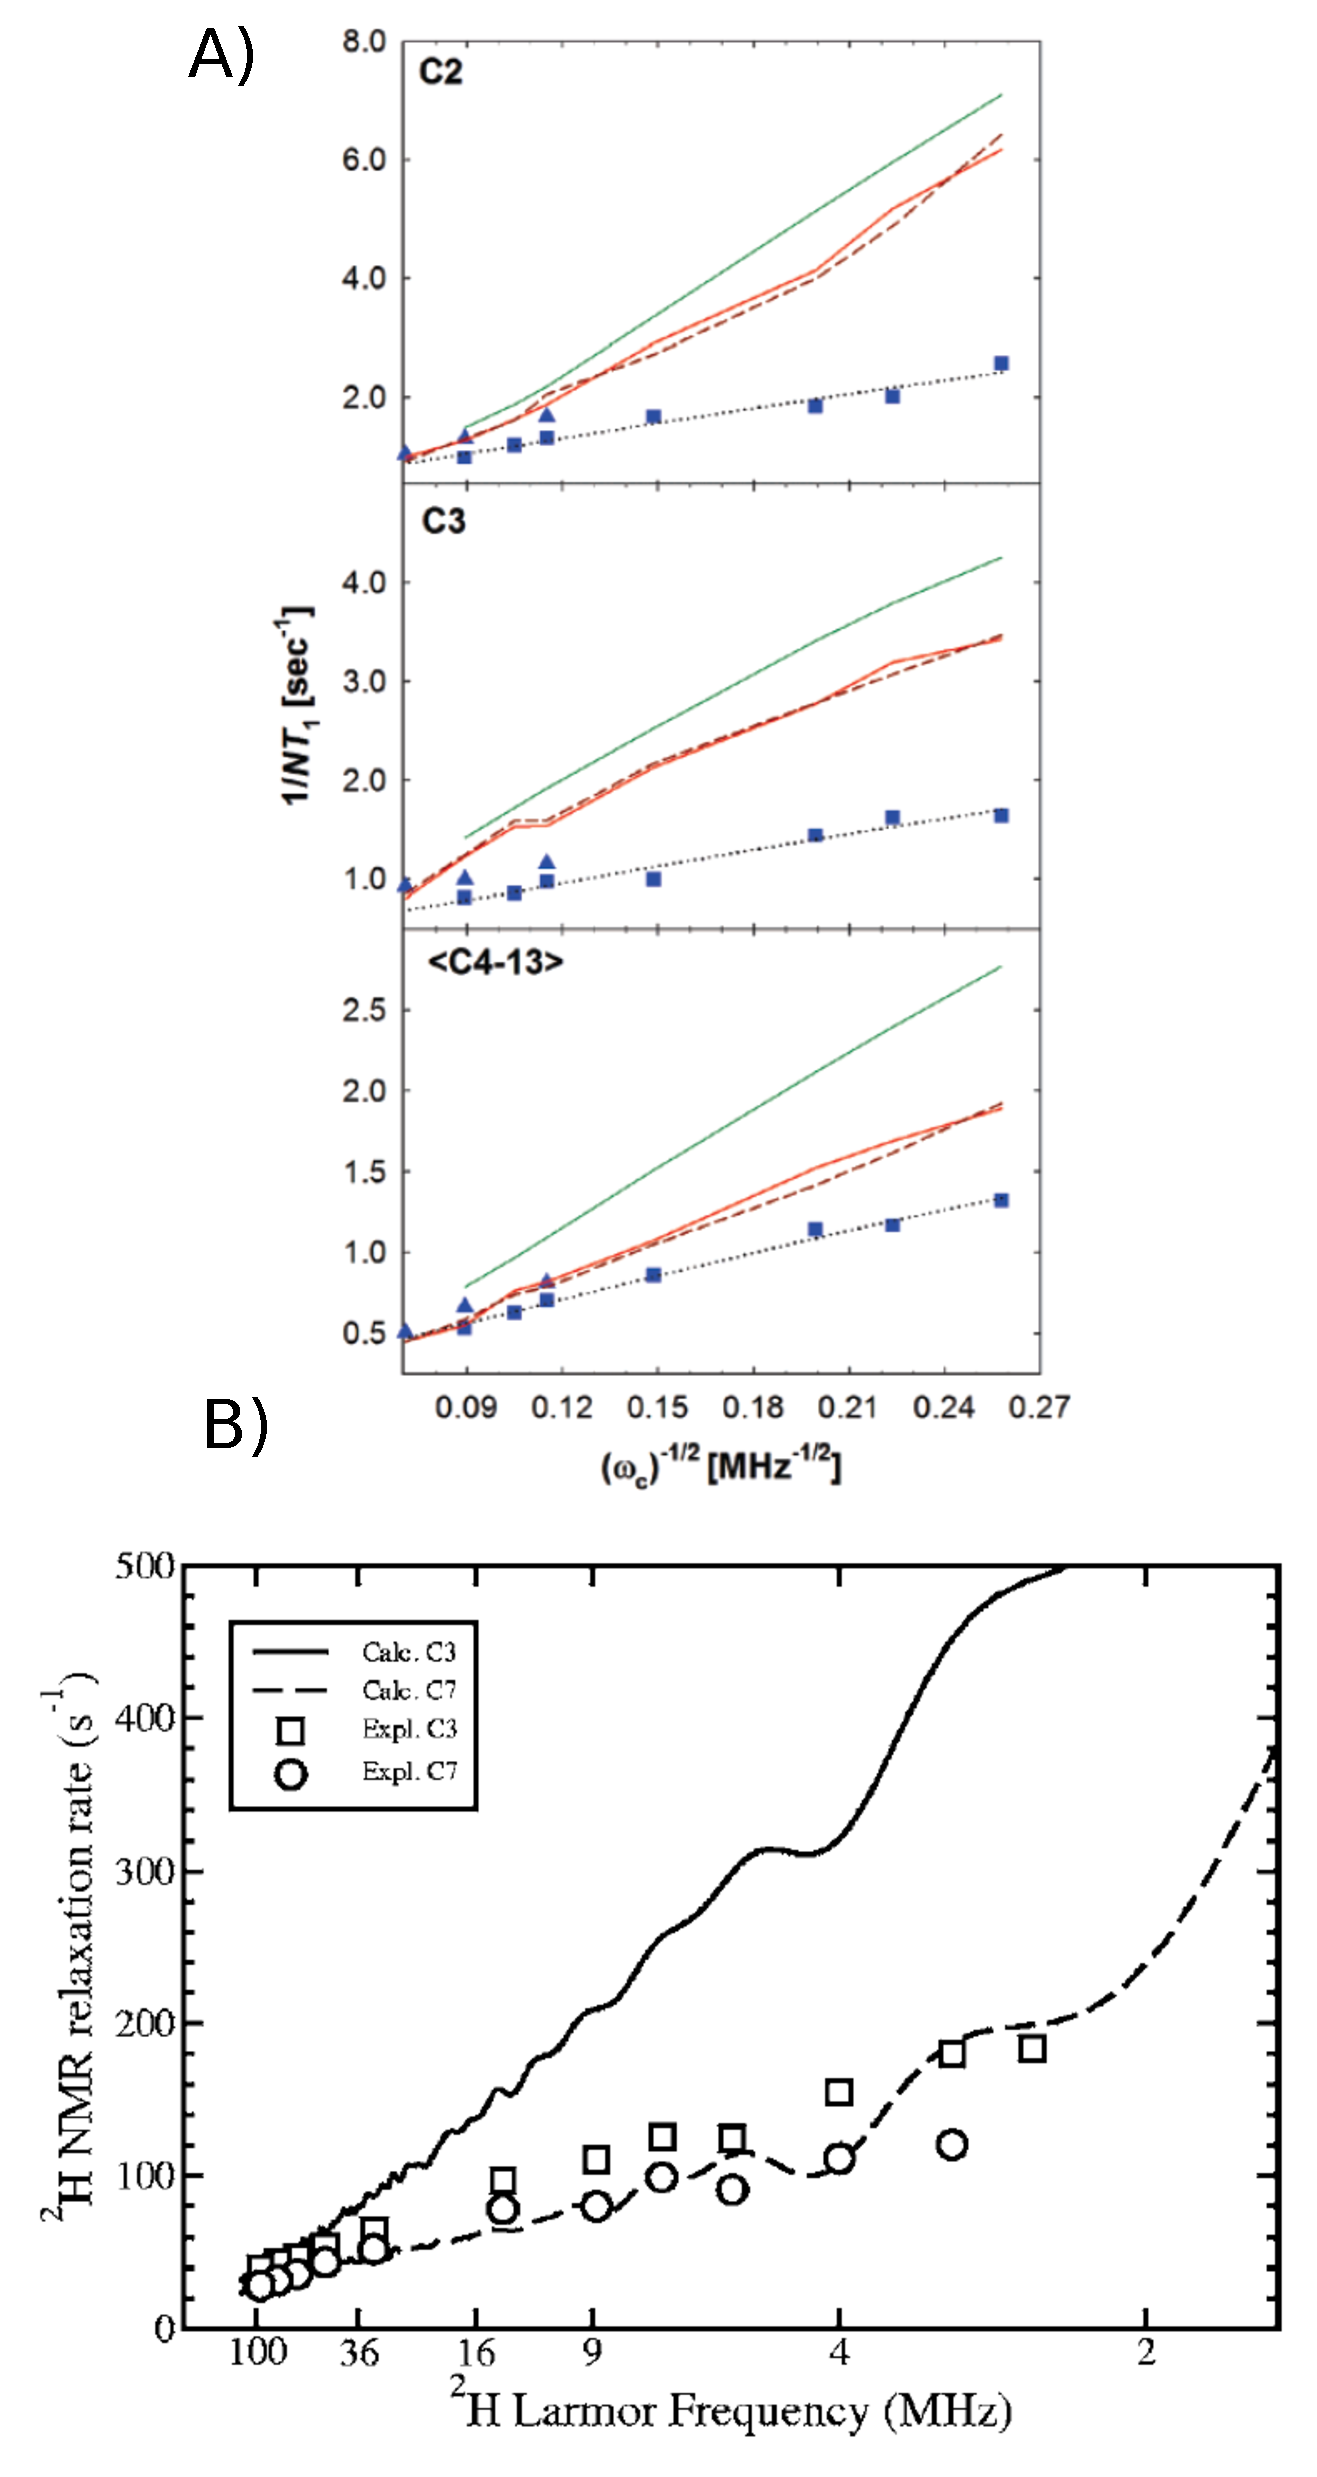
\includegraphics[width=8.6cm]{../Fig/Rdispersion.eps}
\newline
  \caption{\label{Rdispersion}
    A) Comparison of $R_1^{C}$ dependence on magnetic field between experiments and CHARMM simulations for acyl chain carbons (DPPC bilayer in 323K) adapted from~\cite{klauda08a}.
    Experiments as points; MD simulations as solid and dashed lines; and a model-free fit to the vesicle data as dotted lines. 
    B) Comparison of $R_1^{D}$ dependence on magnetic field between experiments and Berger simulations for acyl chain carbons (DMPC bilayer in 300K) adapted from~\cite{wohlert06}.
  } 
\end{figure}
On the other, some studies have compared $R_1^{C}$ and $R_1^{D}$ measured with one magnetic field strenght to the value calculated from
simulations~\cite{feller02,eldho03,ollila07a,klauda08b,klauda12,ferreira15}. Example of such comparison between $R_1^{C}$ from simulations and experiments is shown in Fig.~\ref{RandEFFCT}
\begin{figure}[]
%  \centering
  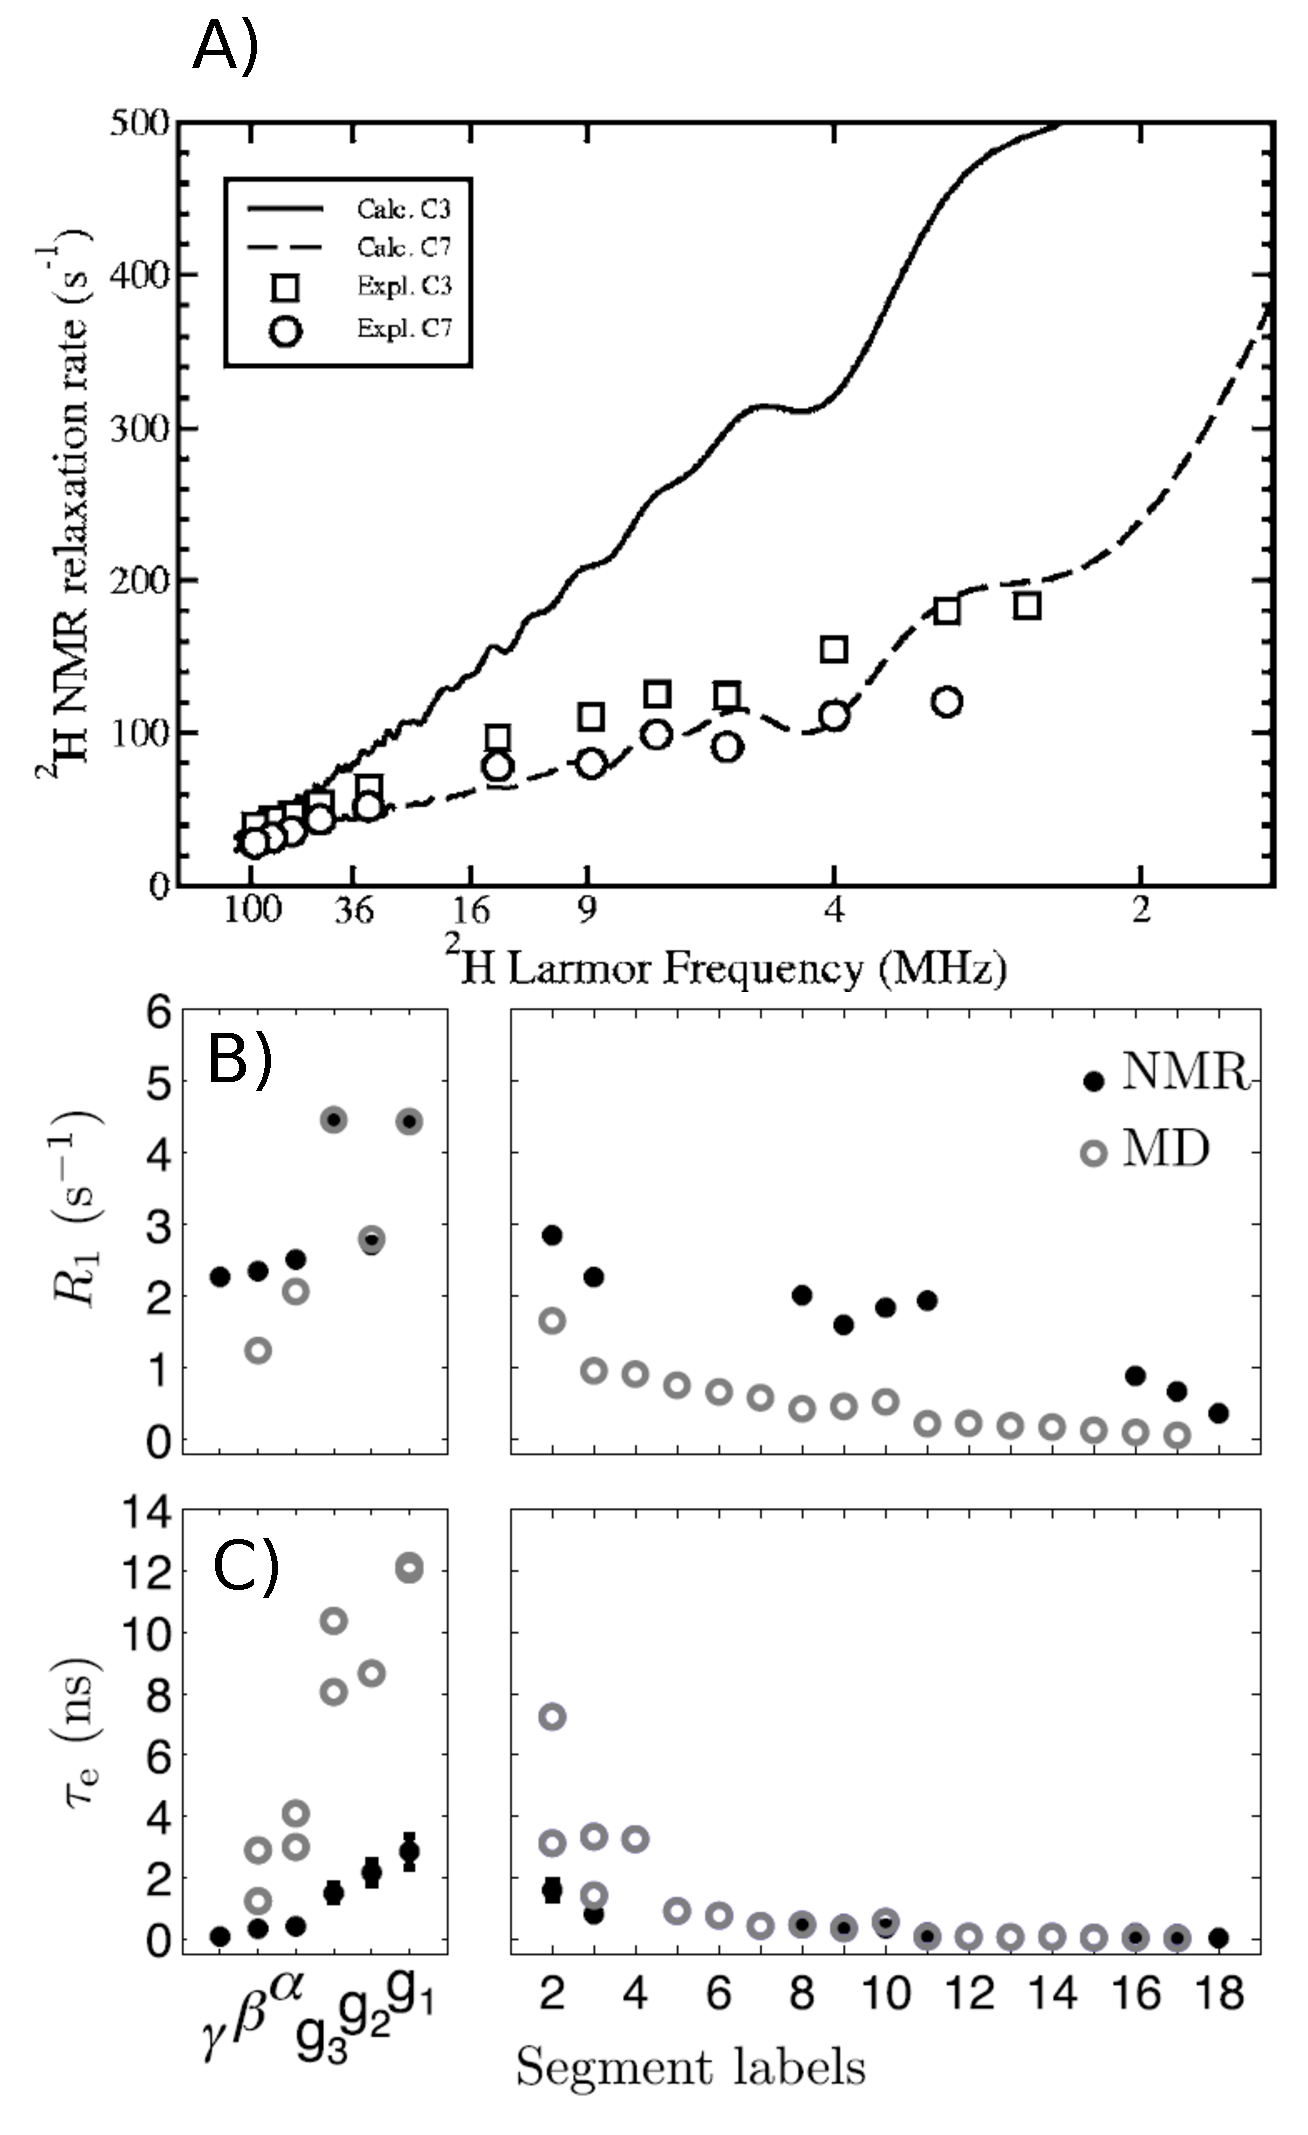
\includegraphics[width=8.6cm]{../Fig/RandEFFCT.eps}
\newline
  \caption{\label{RandEFFCT}
    (top)  $R_1^{C}$ for POPC bilayer in 298K calculated from simulations with Berger model compared to experimental results measured 
    with field strength correspondin to the Larmor frequency of 125 MHz for $^{13}$C.
    (bottom) Effective correlation times for the same system compared between simulations and experiments. 
    Figure adapted from Ferreira et al.~\cite{ferreira15}.
  } 
\end{figure}
Comparisons seems to generally show a good agreement with large larmor frequencies which
is getting worse when the Larmor frequency decreases. On the other hand, the level of the 
agreement depends on the carbon segment and the type of relaxation used in the comparison;
Berger model compared with $2$H NMR gives better agreement for C$_7$ segment compared to
C$_3$ (Fig. \ref{Rdispersion} B)) while comparison to $ 13$C NMR relaxation with one frequency 
gives similar discrepancy for both segments (Fig. \ref{RandEFFCT}). For CHARMM the agreement
seems better when going towards bilayer center, see Fig. \ref{Rdispersion} A).
Due to the complicated connection between molecular dynamics and spin relaxation it
is not straightforward to make conclusions about the dynamical differences between reality
and simulations. This is, however, possible with careful analysis as discussed in the next section.

To ease the intuitive interpretation of experimentally measured rotational dynamics
Ferreira et al. showed that the effective correlation time can be measured by combining 
directly measurable quantities without any assumptions on dynamical prosesses present in the 
fast relaxation regime~\cite{ferreira15}. 
%It should be noted that a quantity called by 
%authors as effective correlation or $\tau_e$ has been reported also previously in the 
%literature, however, these studies typically assume correlation function to have a single
%exponential form \cite{??}. 
%Since molecular dynamical simulations and theoretical understanding
%indicate that assuming a single exponential decay is not realistic, the effective correlation
%times measured with this assumption should not be quantitatively compared to MD simulations
%where multiexponential decay has been observed. The approach by Ferreira et al. is model
%free in the sense that nothing is assumed about the short timescale correlation processes
%when $\tau_e$ is measured \cite{ferreira15}. 
The comparison of effective correlation times
between experiments and simulations for different segments is shown in Fig.~\ref{RandEFFCT}.
From this result it is straightforward to conclude that acyl chain rotational dynamics 
is generally well described while in the interfacial region, especially in glycerol backbone,
the dynamics is too slow in simulations. It should be noted, however, that the effective correlation
describes the total relaxation over all short timescales present in $g_f(t)$. Even if this is 
correct, the balance between different processes with different relaxatio times may not be
correct. This is actually seen in the acyl chains, where $R_1$ does not perfectly agree with
experiments while $\tau_e$ does.  



\subsection{Interplay between simulations and NMR spin lattice relaxation times: Validation and interpretation of dynamics}

By measuring single spin relaxation time values it is almost impossible to make any conclusions
about molecular dynamics due to their complicated connection through the spectral density.
Even changes of relaxation times cannot be directly related to molecular dynamics without further
information since, e.g. faster dynamics may lead to the decrease or increase of spin relaxation times,
depending on the other dynamics processes present and the used magnetic field strength as demonstrated, for example in~\cite{ferreira15}.

Careful studies of spin relaxation times as a function of temperature and magnetic field to overcome this issue are 
recently reviewed by Leftin and Brown~\cite{leftin11}. From compilation of different experimental data sets it was possible 
to conclude, for example, that the interfacial region of lipid molecules has slower dynamics than acyl chains~\cite{leftin11}.
Another successfull approach to interpret the spin relaxation times has been to use the atomistic resolution molecular dynamics
simulations to reproduce the measured changes and then analyze the dynamical changes from the simulation trajectory~\cite{feller02,eldho03,nowacka13}.
This approach has been especially useful in the studies of polyunsaturated acyl chain dynamics which concluded
by combining the simulation and NMR relaxation data that the double bonds speed us the chain dynamics
due to flexible dihedrals next to the double bonds~\cite{feller02,eldho03,gawrisch03,stillwell03}.

To ease the interpretation of the measured spin relaxation times Ferreira et al. recently introduced a model
free connection between effective correlation time and directly measurable spin relaxation rates~\cite{ferreira15}.
The main advantages of effective correlation time is that its connection to molecular dynamics is straightforward in
the sense that the general dynamics is faster when effective correlation time decreases and {\it vice versa} and
that it can be quantitatively compared to simulations. As shown in Fig.~\ref{RandEFFCT} these experiments
immediately show that the glycerol backbone has the slowest dynamics of lipid segments (in agreement with conclusions from the
combination of several previous experimental sets~\cite{leftin11}) and that the dynamics
of these is significantly underestimated by the Berger model.

Most importantly, the rough agreement of spin relaxation rates and effective correlation times between 
simulations and experiments shows that the rotational dynamical processes present in simulations has the 
correct order of magnitude~\cite{pastor88,lindahl01,pastor02,klauda08a,klauda08b,wohlert06,feller02,eldho03,ollila07a,klauda08b,klauda12,ferreira15}. 
Consequently, the dynamical visualizations of simulation trajectories 
(videos) can be considered as a realistic intuitive presentations of lipid bilayers. However,
in more detailed studies it should be kept in mind that all the dynamical (and also structural) details
are not exactly correct. 

The lipid rotational dynamics has been often interpreted by using the so called wobble in the cone model~\cite{pastor88,pastor02,klauda08a,klauda08c,sivanandam09}.
The main idea of the model is that the whole lipid molecule is wobbling as a cone such that all the
all the segments share the time scale for this wobbling. In addition, each segments have further timescales
related to their dynamincs inside the cone. The auto--correlation functions assuming the wobble in the cone
model can be nicely fit to the simulation data and also some experimental results can be reproduced. 
However, also auto--correlation functions having different type of dynamics can be used to do the same.
On the other hand, it has been recently pointed out that significant changes of structure and dynamics 
experienced in acyl chain region may not reflect to the headgroup~\cite{ferreiraTHESIS,botan15} indicating weak coupling 
between these segments. This idea is also in line with one possible interpretation of recent field cycling experiments~\cite{roberts09}.
In addition, the role of undulations in the relaxation data measured with low frequencies is under discussion~\cite{leftin11,edholm08,klauda08a,klauda08c}.

In conclusion, the timescale of rotational dynamics is correct in simulations while the exact correlation times
and relaxation processes are not fully reproduced. More experimental and simulation studies are needed 
to fully understand current quality of dynamics in current models. To interpretate the relaxation prcosesses
present in lipid bilayer, a model which can be shown to agree with experiments on all fast timescales is needed.




%\newpage


\section{Stucture factors from scattering and simulations}

\noindent {\bf For this section I would be more than happy for some help} \\[0.1cm]

\subsection{Form factor measured with X-ray or Neutron scattering}

In scattering experiments the scattering intensity $I(q)\sim|F(q)|^2S(q)$ is observed,
where $F(q)$ is the form factor and $S(q)$ is the structure factor. In the case of lipid
bilayer the structure factor describes the structure of lamellar sheets and the form factor
describes the internal structure of lipid bilayers. The structure factor depends on the
topological phase of lipids and can be considered to be practically constant for unilamellar
vesicles while in multilamellar phase its form is known. Thus, in practise direct
information about form factor is achieved from the measured scattering intensity.

Following the notation from Ref. \cite{kucerka10}, the form factor can be written as 
\begin{equation}\label{FF}
|F(q)|=|\int_{-D/2}^{D/2}(\sum_\alpha f_\alpha(q_z)n_\alpha(z) - \rho_s)(\cos(zq_z) + i \sin(zq_z)) {\rm d}z|,
\end{equation}
where $n_\alpha(z)$ in the atom $\alpha$ number density as a function of membrane normal coordinate $z$,
$f_\alpha(q_z)$ is the scattering length density, $\rho_s$ is the solvent scattering lenght density
and integral spans over bilayer with total thickness $D$.
Neutron scattering length density or X-ray atomic form factors are used for $f_\alpha(q_z)$ depending
on the used scattering technique. The values for these are available in the literature \cite{??}.
The last term disappears for symmetric bilayer but not for asymmetric \cite{??}.
If bilayer symmetry and delta functions for electron densities around atom center are assumed, the Eq. \ref{FF}
becomes to the commonly used form for x-ray scattering
\begin{equation}\label{FFsimpl}
|F(q)|=|\int_{-D/2}^{D/2}\Delta \rho_e(z) \cos(zq_z) {\rm d}z|,
\end{equation}
where $\Delta \rho_e(z)$ is the difference between solvent and the total electron densities.

The form factor can be measured from unilamellar vesicles, multilamellar vesicles or from order bilayer samples. 
The results from samples with different topologies are in good agreement, indicating that the bilayer
structure is similar independently of the lamellar phase topology~\cite{kucerka05,kucerka07}.
Different sample topologies gives the highest resoution with different $q$ ranges,
thus the combination of form factors measured from different topologies are of the used
to maximize the available form factor information~\cite{kucerka05}. In addition, the neutron scattering
resolution is highest with small $q$ values this giving more accurate on longer scales in real spave, like 
on bilayer thickness \cite{??}. On the other hand, x-ray scattering has larger resolution with larger $q$ values
thus giving more accurate information on fine details of the bilayer density profile. Consequently,
the neutron and x-ray scattering measurements complement each others and the combining the information
from both gives the most comprehensible picture on bilayer strucuture~\cite{kucerka08a}.

Form factors are quite accurate given that experimental care has been taken. A delicate issue 
can be subtraction of background (from water and capillary).  \\

\onecolumngrid
\todo{Discussion about related issues can be found at:
{\tt https://github.com/NMRLipids/NMRLipids\_V-Review/issues/1}}


\todo{The discussion is going in at: \\
{\tt https://github.com/NMRLipids/NMRLipids\_V-Review/issues/2} \\
Key questions now:\\
Do we get independetly measured Form Factors plotted to the same figure? \\
Are there good references for the accuracy?
}
\twocolumngrid

\subsection{Form factor calculation from simulations}
To calculate the scattering form factors from simulations the number density from
simulations can be substituted into Eq. \ref{FF}. In the case of neutrons the scattering 
length densities $f_\alpha(q_z)$ are assumed not to depend on $q$ and numerical are usually 
taken from \cite{??}. For x-ray scattering it is often assumed that all electrons pointwisely 
located in the atom position in simulation~\cite{??}. Also in most simulations the bilayer is symmetric,
thus the electron density is simply calculated and substituted into Eq.~\ref{FFsimpl}. 
On the other hand, in some studies gaussian distribution for electrons around atom positions~\cite{benz05} 
or analytical expression for atom scattering length density $f_\alpha(q_z)=\sum_{j=1}^4a_je^{-b_j(q/4\pi)^2}+c$
are assumed~\cite{benz05,kucerka10,??}. In the case of the analytical expression the parameters 
$a_j$, $b_j$ and $c$ are taken from~\cite{??}. For example, the widely used SIMtoEXP software is using
the analytical form~\cite{kucerka10}. The effect of these choises on electron density profiles was discussed
by Benz et al.~\cite{benz05}, however, it is not clear how significant this is when form factors are
compared between simulations and experiments.

The small bilayer patches used in simulations might depress bilayer undulation modes which are present in large 
scale experiments~\cite{braun11}. Braun et al. showed that undulations seen in large enough simulations do
not change the locations of form factor minimaz but depress the peak hights in the lobes~\cite{braun11}.
Since the undulations are expected to be present in the experiments, the potential discrepancies 
between simulations and experiments in the lobe heights may be explained by the lack of undulation 
motions in experiments.

The simulations give the form factors on absolute scale while experiments obtain them only on relative scale,
thus the experimental form factors from different sources has to be scaled for comparison~\cite{kucerka08a,kucerka10}.
In SIMtoEXP program the scaling is performed using the scaling factor $k$ determined from equation
\begin{equation}
k=\frac{\sum_{i=1}^N\frac{|F_s(q_i)||F_e(q_i)|}{(\Delta F_e(q_i))^2}}{\sum_{i=1}^N\frac{|F_e(q_i)|^2}{(\Delta F_e(q_i))^2}},
\end{equation} 
where $F_e(q)$ and $F_s(q)$ are experimental and simulated form factors, respectively, $\Delta F_e(q)$ is the uncertainty
of the experimental form factor and the summation goes over all $N$ data points~\cite{kucerka08a,kucerka10}.
In many studies which compare the form factors between experiments and simulations, the details on the scaling
factor used is not given~\cite{??}. 

\onecolumngrid
\todo{More discussion at: \\
{\tt https://github.com/NMRLipids/NMRLipids\_V-Review/issues/3} \\
and \\
{\tt https://github.com/NMRLipids/NMRLipids\_V-Review/issues/4} \\
I still think that I have seen undulation correction for experimental data mentioned in the literature.
}
\twocolumngrid

\subsection{Interplay between simulations and scattering experiments: Validation and interpretation}
Similarly to NMR order parameters, the form factor gives accurate information about lipid
bilayer structure but the structure cannot be uniquely resolved from the experimental data only.
To give structural intepretation of order parameters, the model for sampled conformations of 
single molecules are needed while to interpret the scattering form factor data the model
for the atom number densities, $n_\alpha(z)$ in Eq.~\ref{FF}, is needed.
Several models developed and used for this purpose are reviewed by Heberle et al.~\cite{heberle12}.

Similarly to the NMR order parameters, also MD simulations can be used in the structural
interpretation if they reproduce the experimental form factors. And in turn,
if simulation model do not reproduce the experimental form factor its structure is not 
realistic. The comparison between experimental and simulated form factors has been done 
in several studies for both purposes, to validate the simulations 
model~\cite{hogberg08,chiu09,klauda10,dickson12,jambeck12,lim12,klauda12,jambeck13,chowdhary13,lee14,maciejewski14,dickson14,tjornhammar14,madej15,kulig15b} and to intepret the experiments~\cite{sachs03,klauda06,kucerka08a,kucerka08b,braun13}. 
The simulations have been also used to improve the fitting based structural models~\cite{??}.

The comparison to experimental area per molecule values to validate the lipid density simulations~\cite{tieleman97} has
been often replaced nowdays with more direct comparison~\cite{nagle00} using x-ray form 
factors~\cite{hogberg08,chiu09,klauda10,dickson12,jambeck12,lim12,klauda12,jambeck13,chowdhary13,lee14,maciejewski14,dickson14,tjornhammar14,madej15,kulig15b}.
In some studies the comparison is complemented with the comparison to the neutron scattering 
data~\cite{dickson12,jambeck12,lee14,dickson14,tjornhammar14,madej15}
In general the models reproduce form factors in good agreement with experiments, especially with lower $q$ values
indicating that the bilayer dimensions, like thickness, are in good agreement. However, the agreement gets often worse
with higher $q$ 
values~\cite{chiu09,klauda10,klauda12,dickson12,lim12,jambeck12,chowdhary13,jambeck13,lee14,maciejewski14,dickson14,kulig15b,madej15}
indicating some differences in detailed electron density profiles~\cite{??}.
For example of the comparison see Fig. \ref{FFcomp}.
The comparison has been usually done based on visual inspection while also quantitative measure
for simulated form factor is suggested \cite{kucerka10}.
In some studies also fourier transform coeffiecients are compared \cite{benz05,??}
\begin{figure*}[]
%  \centering
  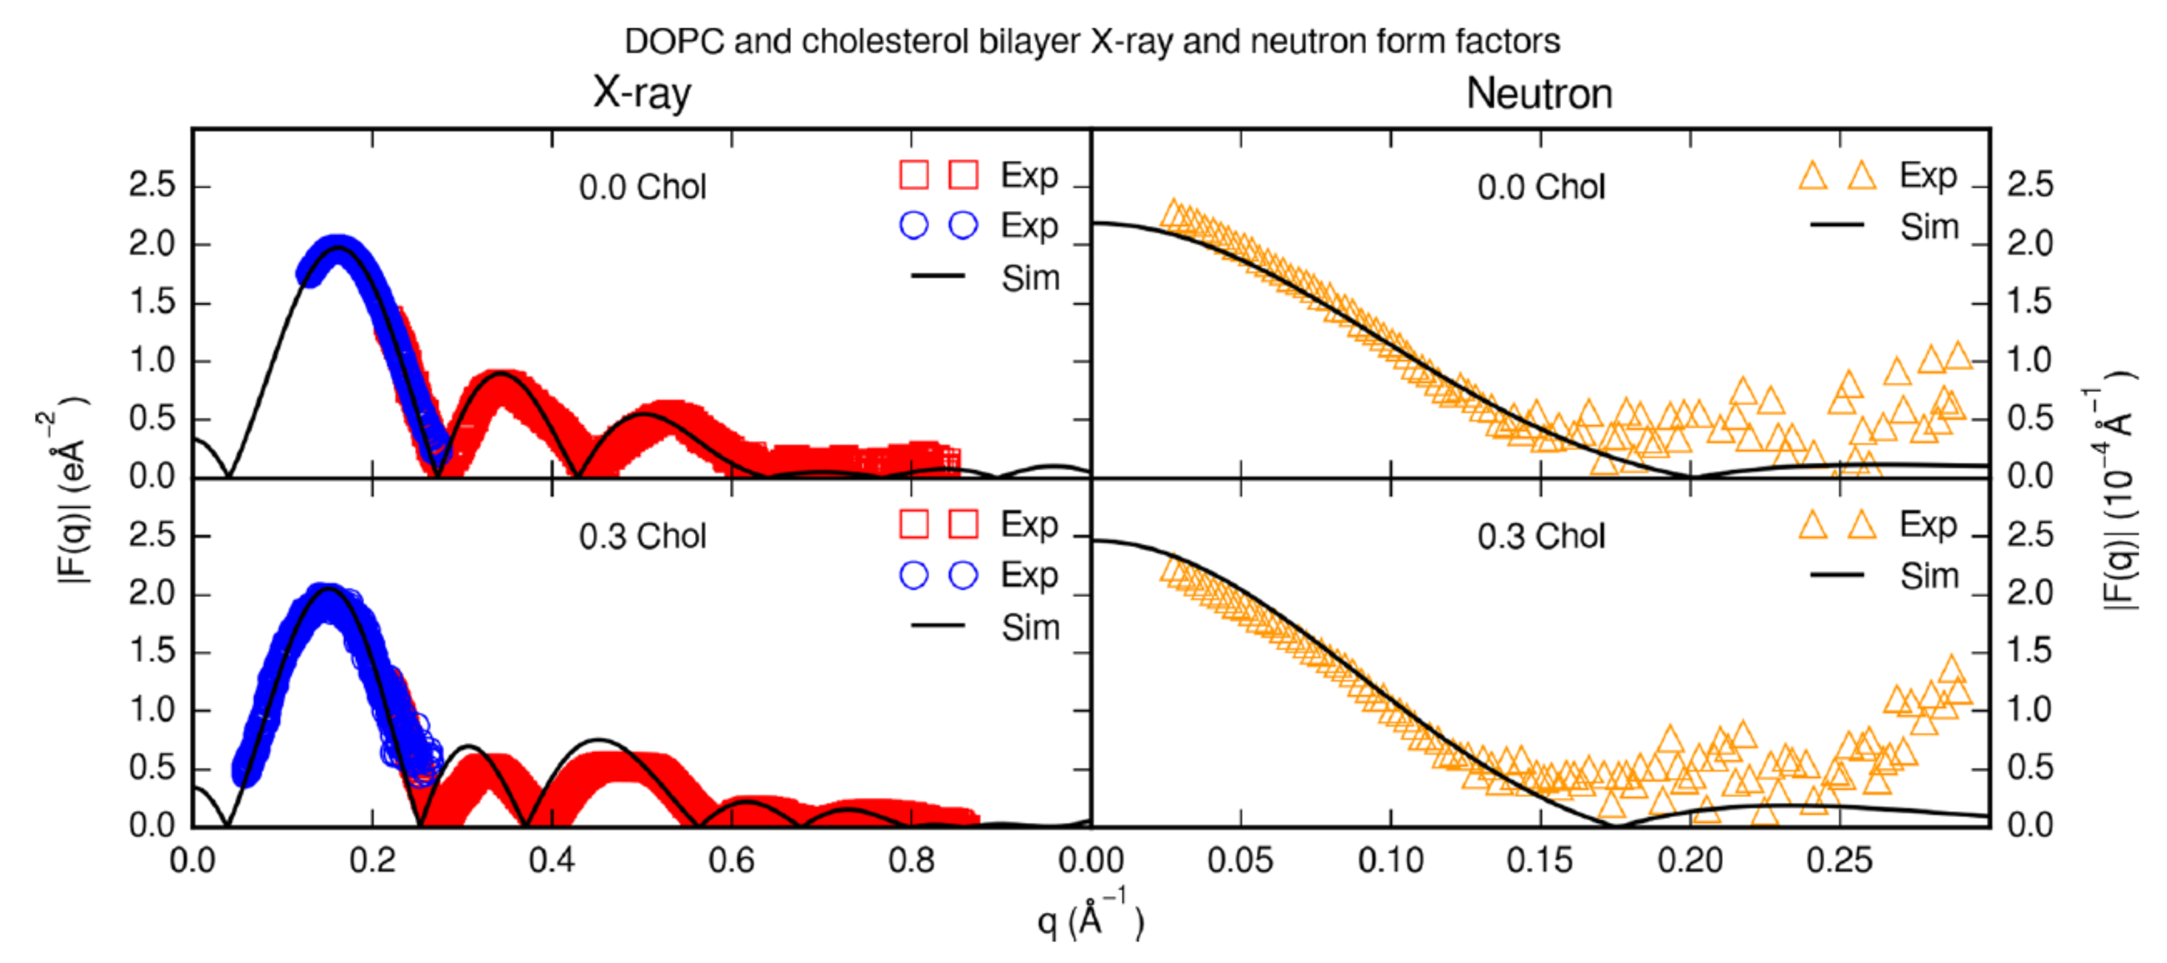
\includegraphics[width=10.6cm]{../Fig/FFcompMADEJ.eps}
\newline
  \caption{\label{FFcomp}
    Example of comparison between simulation model and experiment.
    The agreement is better with low $q$ values and cholesterol induced thickening is overestimated.
    Figure adapted from Madej et al.~\cite{madej15}.
  } 
\end{figure*}


Also changes in form factor due to temperature~\cite{jambeck12,zhuang14}, cholesterol concentration~\cite{jambeck13,madej15} 
and acyl chain polyunsaturation~\cite{eldho03,klauda12} 
has been compared between simulations and experiments~\cite{eldho03,kucerka05,pan08,hodzic08,kucerka08,pan09,khelasvili10,kucerka11}.
Simulation generally reproduce the decreased thickness and increased area with increasing temperature~\cite{jambeck12,zhuang14} and 
polyunsaturation level~\cite{eldho03,klauda12}, 
as well as increased thickness and decreased area with increasing cholesterol concentration~\cite{jambeck13,madej15}.
However, the temperature dependence is underestimated for some systems~\cite{jambeck12,zhuang14} while cholesterol
effect is overestimated~\cite{jambeck13,madej15}. Example of such comparison is shown in Fig. \ref{FFcomp}.

In studies where the main goal is to interpret the form factors using MD simulations instead of validating the model,
the area per molecule is often fixed to a certain value in order to reproduce the experimental form factor 
better~\cite{sachs03,klauda06,kucerka08a,kucerka08b,braun13}.
With this contaraint is indeed, possible to get the form factors close to the experiments, however, 
careful comparisons between experimental form factors, MD simulations and SDP model suggest small but measurable 
structural differences~\cite{kucerka08a,braun13}. The form factor from the SDP model is in better agreement
with simulations and the extracted stuctural parameters indicate differences especially in the headgroup region~\cite{kucerka08a,braun13} 
which is in agreement with the comparions between simulations and NMR order parameter indicating issues in the same region~\cite{botan15}, 
see also section~\ref{??}.

In conclusion, all the state of the art simulation models gives form factors close to experimental
data in various conditions indicating that the average bilayer dimensions are in good agreement with simulations
and experiments. Also the qualitative changes are reproduced, however, sometimes over-or underestimated.
In general, the conclusions from scattering data agrees with conclusions from NMR data:
the hydprohopic acyl chains are often well described in simulations, while in glycerol backbone and headgroup 
regions there is room for improvement.

\onecolumngrid
\todo{The more detailed discussion can be found at: \\
{\tt https://github.com/NMRLipids/NMRLipids\_V-Review/issues/5}}
\twocolumngrid


\section{Conclusions}

Recent studies quantitatively comparing atomistic resolution structure and dynamics of lipid
bilayer between experiments using C--H bond order parameters, spin relaxation rates and
scattering form factors are reviewed. The purpose of these studies is to quantify the atomistic
resolution structural and dynamical quality of simulation models as well as to give an 
atomistic resolution interpretation for the experimental results. For interpretation of
these experiments the atomistic resolution MD simulations reproducing all the experiments would be
an ultimate tool since the same model can be used to interpret all the experiments. For the same 
reason, this atomistic resolution model would be most likely a realistic representation for
atomistic resolution strucutre and dynamics of lipid bilayers. The main conclusion of this
review is that the current MD simulations are not quite yet on the level to perform this task,
however, in several aspects indicate that there is potential to improve the models to become 
truly realistic atomistic resolution representations of these systems. 

More specific conclusions are the following: \\
- The order parameters for each C--H bond in lipid molecules in bilayers can be measured
with high quantitative accuracy with both $ 2$H NMR and $ 13$C NMR and this data
is available for wide range of lipids in different conditions. Comparison of this data to simulations
gives a very detailed picture about the quality of sampled atomistic resolution structures
in lipid bilayer and may also help in structural interpretation of experiments. 
The order parameter changes with varying conditions can be used to study and compare structural changes
between simulations and experiments.\\
- The main conclusions from the comparison of order parameters between experiments and simulations are:
1) the acyl chain structures are generally described realistically for PC lipid bilayers in simulations, 
2) the changes in acyl chain region are qualitatively correct but not always quantitatively,
3) the glycerol backbone and choline structures are not within experimental error for any available model and
4) the results depending on structure and energetics of these sections, like ion binding and lipid--cholesterol interactions
should be taken with caution. \\
- The C--H bond rotational dynamics has correct timescale in simulations models for which comparison has been done.
Most likely the same applies for all models. However, more careful comparison reveals that, e.g. the
glycerol backbone dynamics is too slow in Berger model. Also for CHARMM model all relaxation prosess
do not seem to correctly described. \\
- The development in the scattering methodology has allowed the direct comparison of whole bilayer 
structure between experimental form factor and simulations. This is complementary to the NMR order parameter
which are related to the sampled structures of individual molecules. These comparisons show that the
structural lipid bilayer properties like thickness and area per molecule are close to real values, however,
it seems that there is room for improvement especially in the lipid headgroup region, in agreement with conclusions
from NMR experiments.  

When applying lipid bilayer simulations to study complicated biochemical systems it is crusial to recoknize 
potential artefacts arising from the inaccuracies revealed by these comparisons. Hyphotetical example of
a situation where artificial conclusions might be difficult to avoid would be study of protein approaching
PC lipid bilayer in physiological NaCl concentration. If the above mentioned issues are not carefully taken
into account one might choose a model where the protein is approaching an effectively positively charged 
lipid bilayer due to artificial Na$ +$ binding with incorrect choline structure. In addition to
this the protein might be incorrectly folded already in the bulk water \cite{??}.





% Tables may be be put in the text as floats.
% Here is an example of the general form of a table:
% Fill in the caption in the braces of the \caption{} command. Put the label
% that you will use with \ref{} command in the braces of the \label{} command.
% Insert the column specifiers (l, r, c, d, etc.) in the empty braces of the
% \begin{tabular}{} command.
%
% \begin{table}
% \caption{\label{} }
% \begin{tabular}{}
% \end{tabular}
% \end{table}

% If you have acknowledgments, this puts in the proper section head.
\begin{acknowledgments}
% Put your acknowledgments here.
\end{acknowledgments}

% Create the reference section using BibTe
\bibliography{refs.bib}

%\newpage
%\section{APPENDIX: The NMR results reported by Tiago Ferreira}
\onecolumngrid
\listoftodos

\end{document}
%
% ****** End of file aiptemplate.tex ******
